% Szablon do pracy inżynierskiej, zgodny z Załącznikiem nr 1 do Zarządzenia Rektora PG nr 17/2014 z 1 kwietnia 2014 r. 
% Autor: Mateusz Kraiński
% Kontakt w razie pytań: mt.krainski@gmail.com
% 
% Poza ustawieniem formatowania... wszystkiego, dodano metody ułatwiające właściwe formatowanie niektórych elementów kluczowych. Polecam zapoznać się z tym co jest dostępne.
% 
%
%
%
%
%
% Umieszczenie początku rozdziału, sekcji wraz z nazwiskiem autora w spisie treści.
% \namedchapter[imię i nazwisko autora fragmentu]{Tytuł fragmentu}
% \namedsection[imię i nazwisko autora fragmentu]{Tytuł fragmentu}
% \namedsubsection[imię i nazwisko autora fragmentu]{Tytuł fragmentu}
%
% Przykład:
% \namedchapter[Mateusz Kraiński]{Wstęp i cel pracy} %-> z nazwiskiem
% \namedchapter{Wstęp i cel pracy} %-> bez nazwiska
% 
%
%
%
%
%
% Dodanie wykazu najważniejszych oznaczeń i skrótów. Lista jest automatycznie sortowana osobno dla oznaczeń matematycznych i skrótów:
% \begin{sortedlist}
%  	 \mathitem{symbol}{opis}             %Dodanie elementu - symbolu matematycznego
%  	 \shortitem{Skrót}{wyjaśnienie} 	 %Dodanie elementu - skrótu
%\end{sortedlist}
%  
%Przykład:
%\begin{sortedlist}
%  	 \mathitem{$f_p$}{częstotliwość próbkowania [Hz]}
%  	 \mathitem{$h_m$}{odpowiedź impulsowa pomieszczenia dla $m-$tego mikrofonu}
%  	 \shortitem{RIR}{Room Impulse Response}
%  	 \mathitem{$h_y$}{odpowiedź impulsowa układu $y$}
%\end{sortedlist}
% 
%
%
%
%
%
% Dodanie obrazka w sposób łatwy (jest wpisana ścieżka obrazków jako rys/, czyli należy stworzyć folder 'rys' w folderze, w którym są pliki główne i tam umieszczać obrazki). Ewentualnie można wywołać \graphicspath{ {"ścieżka_dostępu_do_plików"/} } i zmienić ścieżkę dostępu. 
%Metoda może stwarzać problemy ze względu na sposób generacji labelów -> nie są one widoczne przez program, więc nie działa podpowiadanie. Są one tworzone przy kompilacji. Możemy się do nich odwołać przez \ref{fig:label_obrazka}
%
% \InsertImageSimple[rozmiar]{nazwa_pliku}{tytuł}{label_obrazka} -> wstawiany obrazek ma rozmiar 0.0-1.0 szerokości linii (parametr rozmiar w zakresie 0.0-1.0)
% 
% \InsertImageSimple{nazwa_pliku}{tytuł}{label_obrazka} -> wstawiany obrazek ma rozmiar oryginalny
%
% Wstawianie obrazka "the hard way":
%
%\begin{figure}[h!tb]
%	 \centering
%	 
\includegraphics[width = 1.0\linewidth]{logoPG}
%	 \caption{logo PG}
%	 \label{fig:labPG}
%\end{figure}
% 
%
%
%
%
%
% Dodanie dwóch obrazków obok siebie, zasady podobne jak wyżej.
% \InsertSubImagesSimple
%	{nazwa_pliku_obrazek1}
%	{tytuł_obrazek1}
%	{label_obrazek1}
%	{nazwa_pliku_obrazek2}
%	{tytuł_obrazek2}
%	{label_obrazek2}
%	{tytuł_całość}
%	{label_całość}
%
% Przykład z wykorzystaniem obrazków logoETI i logoPG tworzy etykiety fig:ETI, fig:PG i fig:logos:
% \InsertSubImagesSimple
%	{logoETI}		%nazwa_pliku_obrazek1
%	{ETI}			%tytuł_obrazek1
%	{ETI}			%label_obrazek1
%	{logoPG}		%nazwa_pliku_obrazek2
%	{PG}			%tytuł_obrazek2
%	{PG}			%label_obrazek2
%	{Loga}			%tytuł_całość
%	{logos}			%label_całość
%
% Dodanie obrazków obok siebie "the hard way". Proszę korzystać z realCaptionx i tam wpisywać tytuły obrazków ze względu na wymagane formatowanie. Można powiedzieć, że to wersja beta - nie było za bardzo testowane, ale działało:
% 
% \begin{figure}[h!tb] 
%	\centering
%   \def\realCaptionA{tytuł_obrazek1}
%	\def\realCaptionB{tytuł_obrazek2}
%	\def\realCaptionAll{tytuł_całości}
%	\begin{subfigure}[t]{0.4\linewidth}
%		\caption{)}
%		\centering
%		\includegraphics[width = 1.0\linewidth]{plik_obrazek1}
%		\label{fig:lab1}		
%	\end{subfigure}
%	\quad
%	\begin{subfigure}[t]{0.4\textwidth}
%		\caption{)}
%		\centering
%		\includegraphics[width = 1.0\linewidth]{plik_obrazek2}
%		\label{fig:lab2}
%	\end{subfigure}
%	\def\showncap {\realCaptionAll\\ a) \realCaptionA, b) \realCaptionB}
%	\caption[\realCaptionAll]{\showncap}
%	\label{fig:labc}
% \end{figure}
% 
%
%
%
%
%
% Dodanie opisu zmiennych do równania \equationDescriptor i \equationDescriptorS. Druga funkcja dodatkowo sortuje alfabetycznie podane symbole (może to być przydatne przy skomplikowanych wzorach, ale nie przydatne przy prostych, gdzie zmienne podajemy w porządku pojawiania się). Składania podobna jak w sortedList, ale jest trochę inne formatowanie wynikowe.
%
% \begin{equationDescriptor}
% 	\EQDitem{symbol}{opis} -> EQation Descriptor item
% 	\EQDitem{symbol}{opis} 
% \end{equationDescriptor}
%
% Przykład:
% \begin{equation}
% 	s = v_0 \cdot t + \frac{a\cdot t^2}{2}
%   \label{eq:my_eq}
% \end{equation}
% gdzie:   				% nie należy zostawiać linii wolnej przed "gdzie:", gdyż spowoduje to rozpoczęcie tej linii od akapitu
% \begin{equationDescriptor}
%   \EQDitem{$s$}{droga w ruchu prostoliniowym, jednostajnie przyspieszonym [m],}
% 	\EQDitem{$v_0$}{prędkość początkowa [m/s],}
%   \EQDitem{$t$}{czas poruszania się ciała [s],}
% 	\EQDitem{$a$}{przyspieszenie [m/s$^2$ ].}
% \end{equationDescriptor}
% 
%
%
%
%
%
% Tworzenie tabeli. Najtrudniejsza w obsłudze z podanych metod i jest dość trudna w upraszczaniu. Niestety nie działa w 100 procentach jak powinno - nie dzieli tabeli na strony i nie powtarza tytułu tabeli na nowej stronie. Okazało się to zbyt skomplikowane w implementacji i nie było motywacji żeby zrobić to do końca. Jeżeli ktoś chciałby dokończyć - proszę się nie krępować. 
% W linijce \begin{tabularx}{\linewidth}[c]{|l|X|}}, w ostatnich nawiasach klamrowych zdefiniowana jest struktura tabeli (liczba i rodzaj kolumn). W tym przypadku oznacza to jedną kolumnę dopasowaną do szerokości tekstu (oznaczenie l) i jedną kolumnę o maksymalnej pozostałej szerokości (oznaczenie X). W celu stworzenia tablicy trzykolumnowej, o dwóch kolumnach o maksymalnej szerokości należy tam wpisać |l|X|X|. W celu stworzenia tablicy o 4 kolumnach, z czego pierwsza i trzecia mają minimalną szerokość, a pozostałe maksymalną należy wpisać |l|X|l|X| itd.
% W linijkach:
%  	1 & opis1 \\ \hline
%  	2 & opis1\\ \hline
%  	3 & opis1\\ \hline
% są dane do umieszczenia w tabeli. Parametr & oznacza zmianę kolumny, a \\ przejście do nowego wiersza. \hline wstawia poziomą linię oddzielającą wiersze tabeli. Zgodnie z wytycznymi do formatowania powinna być ona obecna.
%
% \begin{table}[h!tb]
% \centering
% \small
% \caption{tutaj_wpisz_tytuł}
% \begin{tabularx}{\linewidth}[c]{|l|X|}} 
%	\hline
%  	1 & opis1 \\ \hline
%  	2 & opis1\\ \hline
%  	3 & opis1\\ \hline
%  	\noalign{\smallskip}
% \end{tabularx}
% \vspace{-8pt}
% \end{table}
% 
%
%
%
%
% Bibliografia znajduje się w pliku bibl.bib. Należy tam dodawać pozycje zgodnie ze standardem bibtex. Jeżeli np. wyszukujemy coś w scholar.google.com klikamy na "Cytuj" pod interesującym nas artykułem, zaznaczamy format BibTeX i kopiujemy całość do pliku bibl.bib
% Obecnie znajduje się tam przykład, do którego w tekście możemy się odwołać przez \cite{labelofarticle}. Pojawi się on w bibliografii dopiero jak zostanie zacytowany, więc nie musimy się przejmować kolejnością wstawiania kolejnych pozycji
% 
%
%
% To już wszystko. W razie pytań poważnie proszę pisać - chętnie pomogę :-) 
% Enjoy! :-)
%
% Testowane na Linuxie Ubuntu 14.10 i jak to powtarzają programiści - U MNIE DZIAŁA!
% U kolegi na Windows 8.1 też :-)


%Plik konfiguracyjny
%Szablon do pracy inżynierskiej 2014
% Autor: Mateusz Kraiński
% Kontakt: mt.krainski@gmail.com


\documentclass[a4paper,twoside,10pt]{report}

\usepackage[a4paper, left=3.5cm, right=2.5cm, top=2.5cm, bottom=2.5cm, headsep=1.2cm]{geometry}
\setlength\parindent{1.25cm}

\usepackage[MeX]{polski} %Mex zawiera polskie fonty
\usepackage[utf8]{inputenc} %kodowanie 1250, dla iso to: "latin2"

% Closest to arial as i could get
\renewcommand{\familydefault}{\sfdefault}
\normalfont

\usepackage{pifont}
\usepackage{float}
\usepackage[pdftex]{graphicx}
\usepackage[nottoc]{tocbibind}
\usepackage{longtable}
\usepackage{enumerate}
\usepackage{fancyhdr}
\usepackage{indentfirst} %do każdego akapitu dodawane jest wcięcie, zgodnie z polskimi standardami drukarskimi.
\usepackage{sectsty}
\usepackage{setspace} %ustawianie interlini, dobrze wygladaja tabele, \singlespacing, \onehalfspacing, and \doublespacing
\usepackage{float}
\usepackage{amsthm} %dla twierdzen
\usepackage{amsmath} %pakiet matematyczny
\usepackage{amssymb} %pakiet dodatkowych symboli
\usepackage{multirow}\usepackage{amsthm} %dla twierdzen
\usepackage{amsmath} %pakiet matematyczny
\usepackage{amssymb} %pakiet dodatkowych symboli
\usepackage{multirow}
\usepackage{xcolor,listings} %listingi
\usepackage[final]{pdfpages}
\usepackage{listings}
\usepackage{url}
\usepackage{tabularx}
\usepackage{gensymb}
\usepackage{textcomp} % promil \textperthousand

\singlespacing
\sectionfont{\large}
\subsectionfont{\normalsize}
\renewcommand{\baselinestretch}{1.0}


%---------------------------------------------------------------------------------
%Sortowanie tekstu
\usepackage{datatool}% http://ctan.org/pkg/datatool

\DTLnewdb{MathSymbols}
\DTLnewdb{Shortcuts}
\newcolumntype{R}{>{\raggedright\arraybackslash}X}

\newcommand{\mathitem}[2]{%
  \DTLnewrow{MathSymbols}% Create a new entry
  \DTLnewdbentry{MathSymbols}{name}{ #1}% Add entry as description
  \DTLnewdbentry{MathSymbols}{description}{#2}
}
\newcommand{\shortitem}[2]{%
  \DTLnewrow{Shortcuts}% Create a new entry
  \DTLnewdbentry{Shortcuts}{name}{#1}% Add entry as description
  \DTLnewdbentry{Shortcuts}{description}{#2}
}
\newenvironment{sortedlist}{%
  \DTLifdbexists{MathSymbols}{\DTLcleardb{MathSymbols}}{\DTLnewdb{MathSymbols}}
  \DTLifdbexists{Shortcuts}{\DTLcleardb{Shortcuts}}{\DTLnewdb{Shortcuts}}
  % Create new/discard old list
  }
  {%
  \DTLsort{name}{MathSymbols}% Sort list
  \begin{flushleft}
  \begin{tabularx}{\linewidth}[c]{l c R}
  \DTLforeach*{MathSymbols}{\theName=name, \theDesc=description}{
     \theName & -- & \theDesc \vspace{6pt}\\}
  \DTLforeach*{Shortcuts}{\theName=name, \theDesc=description}{
     \theName & -- & \theDesc \vspace{6pt}\\}
  \end{tabularx}
  \vspace{-26pt}
  \end{flushleft}
}

\DTLnewdb{eqlist}

\newcommand{\EQDitem}[2]{%
  \DTLnewrow{eqlist}% Create a new entry
  \DTLnewdbentry{eqlist}{name}{#1}% Add entry as description
  \DTLnewdbentry{eqlist}{description}{#2}
}
\newenvironment{equationDescriptorS}{%
  \DTLifdbexists{eqlist}{\DTLcleardb{eqlist}}{\DTLnewdb{eqlist}}
  % Create new/discard old list
  }
  {%
  \DTLsort{name}{eqlist}% Sort list
  \begin{flushleft}
  \vspace{-8pt}
  \begin{tabularx}{\linewidth}[c]{l c R}
  \DTLforeach*{eqlist}{\theName=name, \theDesc=description}{
     \theName &--& \theDesc\\}
  \end{tabularx}
  \vspace{-24pt}
  \end{flushleft}
}

\newenvironment{equationDescriptor}{%
  \DTLifdbexists{eqlist}{\DTLcleardb{eqlist}}{\DTLnewdb{eqlist}}
  % Create new/discard old list
  }
  {
  \begin{flushleft}
  \vspace{-8pt}
  \begin{tabularx}{\linewidth}[c]{l c R}
  \DTLforeach*{eqlist}{\theName=name, \theDesc=description}{
     \theName &--& \theDesc\\}
  \end{tabularx}
  \vspace{-24pt}
  \end{flushleft}
}



%-------------------------------------------------------------sub--------------------
%Formatowanie spisu treści
\usepackage{lipsum}
\usepackage{titlesec}
\usepackage{titletoc}

% Definicja nowego sposobu umieszczania tytułów sekcji
\def\empty{none}
\newcommand{\namedchapter}[2][\empty]{\chapter[#2 \ifx#1\empty\else(#1)\fi]{#2}}
\newcommand{\namedsection}[2][\empty]{\section[#2 \ifx#1\empty\else(#1)\fi]{#2}}
\newcommand{\namedsubsection}[2][\empty]{\subsection[#2 \ifx#1\empty\else(#1)\fi]{#2}}


\titlecontents{chapter}
[0.0cm]             % left margin
{\vspace{6 pt }}                  % above code
{%                  % numbered format
{\thecontentslabel. }%
}%
{}         % unnumbered format
{\enspace\titlerule*{.}\contentspage}         % filler-page-format, e.g dots

\titlecontents{section}
[1em]             % left margin
{\vspace{6 pt }}                   % above code
{%                  % numbered format
{\thecontentslabel. }%
}%
{}         % unnumbered format
{\enspace\titlerule*{.} \contentspage}         % filler-page-format, e.g dots

% indented subsection (in toc)
\titlecontents{subsection}
[2em]             % left margin
{\vspace{6 pt }}                   % above code
{%                  % numbered format
{\thecontentslabel. }%
}%
{}         % unnumbered format
{ \enspace\titlerule*{.}\contentspage}         % filler-page-format





%---------------------------------------------------------------------------------
% Formatowanie rozdziałów, podrozdziałów itd.
\usepackage{textcase}
\usepackage{titlesec}


\titleformat
{\chapter} % command
[hang] % shape
{\bfseries\large} % format
{\thechapter. } % label
{0pt} % sep
{\MakeTextUppercase} % before-code
[] % after-code
\titlespacing*{\chapter}{0pt}{12pt}{6pt}


\titleformat
{\section} % command
[hang] % shape
{\normalsize\bfseries\itshape} % format
{\thesection. } % label
{0em} % sep
{} % before-code
[] % after-code
\titlespacing*{\section}{0pt}{12pt}{6pt}

\titleformat
{\subsection} % command
[hang] % shape
{\normalsize\itshape} % format
{\thesubsection. } % label
{0em} % sep
{} % before-code
[] % after-code
\titlespacing*{\subsection}{0pt}{12pt}{6pt}



%---------------------------------------------------------------------------------
% Change itemize point style
\renewcommand{\labelitemi}{$\bullet$}
\renewcommand{\labelitemii}{$\circ$}
\renewcommand{\labelenumi}{\arabic{enumi}. }
\renewcommand{\labelenumii}{\labelenumi\arabic{enumii}. }
\renewcommand{\labelenumiii}{\labelenumii\arabic{enumiii}. }




%---------------------------------------------------------------------------------

%Change image style, add simple functions InsertImageSimple and InsertSubImagesSimple
%\usepackage{caption}
\usepackage[font=small, labelsep=period, figurename=Rys., aboveskip=6pt, belowskip=0pt]{caption}
\usepackage{subcaption}

\captionsetup*[subfigure]{
	font=small,
	singlelinecheck=off,
	justification=raggedright,
	labelformat=simple,
	labelsep=none,
	aboveskip=6pt,
	belowskip=0pt
}

\graphicspath{ {rys/} }

\newcommand{\InsertImageSimple}[4][\empty]
{
\begin{figure}[h!tb]
    \centering
    \ifx#1\empty\includegraphics[scale=1]{#2}\else\includegraphics[width = #1\linewidth]{#2}\fi
    \caption{#3}
	\label{fig:#4}
\end{figure}
}

\newcommand{\InsertSubImagesSimple}[8]
{
\begin{figure}[h!tb]
	\centering
	\begin{subfigure}[t]{0.4\linewidth}
		\caption{)}
	%	\def\realCaptionA{#2}
		\centering
		\includegraphics[width = 1.0\linewidth]{#1}
		\label{fig:#3}
	\end{subfigure}
	\quad
	\begin{subfigure}[t]{0.4\textwidth}
		\caption{)}
	%	\def\realCaptionB{#5}
		\centering
		\includegraphics[width = 1.0\linewidth]{#4}
		\label{fig:#6}
	\end{subfigure}
	%\def\realCaptionAll{#7}
	\def\showncap {#7\\ a) #2, b) #5}
	\caption[#7]{\showncap}
	\label{fig:#8}
\end{figure}
}

%---------------------------------------------------------------------------------
% Change table style

\captionsetup[table]{
    listformat=empty,
    name=Tabela,
    singlelinecheck=off,
    justification=raggedright,
    labelsep=period,
    position=above,
    aboveskip=0pt,
	belowskip=-4pt,
    width=\linewidth,
    labelfont={small, bf},
    font={small}
    }

%---------------------------------------------------------------------------------
%---------------------------------------------------------------------------------
%Dodatki
\makeatletter
\newcommand{\setappendix}{Dodatek~\thechapter:~}
\newcommand{\setchapter}{\thechapter~}
\titleformat{\chapter}{\bfseries\large}{%
  \ifnum\pdfstrcmp{\@currenvir}{appendices}=0
    \setappendix
  \else
    \setchapter
  \fi}{0em}{}
\makeatother
\usepackage[titletoc, title]{appendix}
\usepackage[justification=centering]{caption}

\renewcommand\appendixname{}
\renewcommand\appendixpagename{Dodatki}
\renewcommand\appendixtocname{Dodatki}


\begin{document}


% Strona tytułowa, 
% Należy podać ścieżkę dostępu do plików pdf zawierających oświadczenie i stronę tytułową. Po dodaniu ścieżki odkomentować linijkę %\pagestyle{empty}
\begin{figure*}[h!tb]
\vspace*{-2.5cm}
\hspace*{-3.5cm}
	\centering
      	\includegraphics{\StronaTytulowa}
\end{figure*}
\clearpage
\newpage
\thispagestyle{empty}
\mbox{}
\pagestyle{empty}
\begin{figure*}[h!tb]
\vspace*{-2.5cm}
\hspace*{-3.5cm}
	\centering
	\includegraphics{\Oswiadczenie}
\end{figure*}
\clearpage
\newpage
\thispagestyle{empty}
\mbox{}
\setcounter{page}{2}
\def\StronaTytulowa{StronaTytulowa_149097.pdf}
\def\Oswiadczenie{Oswiadczenie_149097.pdf}
\pagestyle{empty}
\begin{figure*}[h!tb]
\vspace*{-2.5cm}
\hspace*{-3.5cm}
	\centering
      	\includegraphics{\StronaTytulowa}
\end{figure*}
\clearpage
\newpage
\thispagestyle{empty}
\mbox{}
\pagestyle{empty}
\begin{figure*}[h!tb]
\vspace*{-2.5cm}
\hspace*{-3.5cm}
	\centering
	\includegraphics{\Oswiadczenie}
\end{figure*}
\clearpage
\newpage
\thispagestyle{empty}
\mbox{}
\setcounter{page}{2}

%streszczenie
\chapter*{Streszczenie}

Żyjemy w czasach, w których zewsząd otaczają nas duże zbiory danych i algorytmy uczenia maszynowego.

Myślą przewodnią pracy jest zastosowanie jednego algorytmu sztucznej inteligencji do lepszego doboru parametrów innego programu tego typu.
We wstępie wysunięto tezę główną, tj. że możliwe jest optymalizowanie struktury konwolucyjnych sieci neuronowych za pomocą algorytmu genetycznego.
Teza pomocnicza głosi, że istnieje związek pomiędzy wynikami sieci po jednej epoce uczenia a jej ostatecznymi osiągami.
Została ona wysunięta w związku z potrzebą oszczędności czasu i kosztów obliczeniowych, a uczenie przez jedną epokę pozwala na ich redukcję.


Następnie zgłębione zostały kluczowe dla tego tematu zagadnienia. Poczynając od zdefiniowania pojęć takich jak uczenie maszynowe, meta uczenie czy uczenie z nadzorem,
poprzez przedstawienie problemu klasyfikacji obrazów z przybliżeniem zbioru testowego CIFAR-10, przedstawienie metody k-najbliższych sąsiadów i klasyfikatora liniowego, kończąc
na metodach sztucznej inteligencji takich jak sieci neuronowe, konwolucyjne sieci neuronowe i algorytm genetyczny.

Po zredukowaniu problemu do optymalizacji struktury po jednej epoce uczenia i przedstawieniu pojedynczej sieci neuronowej jako jednego osobnika w algorytmie genetycznym oraz zdefiniowaniu operacji genetycznych
wykonywanych nań, zaprojektowano system do przeprowadzenia eksperymentu.

System został obszernie omówiony, poczynając od węzła zarządzającego, przez system kolejkowania zadań i zaprojektowany protokół komunikacji ze zdalnymi węzłami, po strukturę samego węzła obliczeniowego
i sposób zarządzania owymi węzłami. Omówiono sposób zapewnienia replikacji badań.

Następnie przedstawione są wyniki badań i testów, w tym badanie wariancji pomiaru skuteczności klasyfikacji sieci w zależności od ziarna generatora losowego, przez testowanie działania algorytmu genetycznego i systemu kolejkowego,
po właściwe badania zależności pomiędzy uczeniem krótkim i długim oraz poszukiwania optymalnej struktury. Z badań wyciągnięto wnioski popierające tezy sformułowane we wstępie.

Następnie wyniki są krótko omawiane w podsumowaniu, gdzie również proponowane są dalsze kierunki rozwoju systemu.
\\\\
\noindent
\textbf{Słowa kluczowe}: automatyzacja, sieci neuronowe, algorytmy genetyczne, sztuczna inteligencja
\\

\noindent
\textbf{Dziedzina nauki i techniki, zgodnie z wymogami OECD}: nauki inżynieryjne i techniczne, systemy automatyzacji i kontroli
\chapter*{Abstract}
We live in a time where we are surrounded by Big Data and Machine Learning Algorithms.

The main thought driving this thesis is using an artificial intelligence algorithm for choosing better parameters for another program of the same class.
In the introduction the main thesis is introduced, which states that it is possible to perform optimization of a convolutional network structure using the genetic algorithm.
A supporting thesis states that there is a connection between classification accuracy of a neural network after 1 and after more epochs of training.
The second thesis was a natural consequence of the need to preserve time and computing resources, and 1-epoch training allows that.

Key concepts crucial for proving the thesis have been covered.
Machine learning, meta learning, and supervised learning are defined as first.
Then we move on to elaborate on the image classification problem, the CIFAR-10 dataset, k-nearest neighbor method and linear classifiers.
Finally artificial intelligence concepts such as neural networks, convolutional neural networks (CNNs) and the genetic algorithm are covered.

After reducing the problem to optimizing the structure of a convolutional neural network after 1 epoch of training, defining the specimen in the genetic algorithm as a single CNN structure and specifying the genetic operations of the algorithm, a system for conducting the experiment is proposed.

Further on, the system is broadly discussed, starting with the management node, through the queuing system and a proposed communication protocol for communication with the remote nodes, arriving at the structure of a worker node and a management system for the worker nodes.
A way to ensure reproducibility of the experiment is being introduced.

Finally the experiment and tests results are discussed, including measuring the variance of the classification accuracy of a single neural network trained with different random seeds and testing if the queuing system works properly.
After that the actual experiment results are being discussed, including looking for a connection between long- and short-term training and optimizing the network structure.
The results provide insights supporting both the theses.

Finally the results are shortly discussed in the summary, where possible further system development direction and improvements are proposed.
 \\\\
\noindent
\textbf{Keywords}: automation, neural networks, genetic algorithm, artificial intelligence\\\\
\noindent
\textbf{Field    of    science    and    technology    in    accordance    with    OECD    requirements}: engineering and technology, automation  and  control  systems


%spis treści
\tableofcontents

%wykaz skrótów
%\clearpage
\addcontentsline{toc}{chapter}{Wykaz ważniejszych oznaczeń i skrótów}
\chapter*{Wykaz ważniejszych oznaczeń i skrótów}

%Sortowanie automatyczne, osobno dla skrótów i oznaczeń matematycznych
%Można dodawać w dowolnej kolejności oznaczenia - algorytm sobie z tym poradzi
%Użycie:
%\begin{sortedlist}
% \mathitem{oznaczenie_matematyczne}{wyjaśnienie oznaczenia}
% \shortitem{skrót}{wyjaśnienie skrótu}
%\end{sortedlist}

%Przykład!
\begin{sortedlist}
  \shortitem{KSN}{Konwolucyjna Sieć Neruonowa}
  \shortitem{AG}{Algorytm Genetyczny}
  \mathitem{$\tau$}{Stała czasowa [s]}
\end{sortedlist}


%W pliku Chapter.tex umieszczamy treść pojedynczego rozdziału pracy. Radzę go skopiować tyle razy ile plików będziemy używali. Dzięki zapisywaniu każdego chaptera w osobnym pliku praca jest przejrzysta i łatwo się edytuje czy pracuje nawet w kilka osób, bez specjalistycznego oprogramowania do kontroli wersji.
\chapter{Wstęp}
W dobie powszechnego dostępu do internetu i informatyzacji człowiek produkuje olbrzymie ilości danych.
Każdego dnia setki milionów ludzi robi zdjęcia, tworzy filmy i wysyła wiadomości tekstowe.
Rządy państw regularnie zbierają dane wszelkiego rodzaju, od spisów statystycznych po raporty incydentów od jednostek policji.
Ogrom tych danych rośnie w dużym tempie.
Całkowita liczba danych na świecie wyniosła 4.4 zettabajtów ($4.4 * 10^{21}$) danych.
Prognozuje się dalszy wzrost do 44 zettabajtów do roku 2020.
Szacuje się, że dziennie powstaje ok. 2,5 exabajtów ($2,5 * 10^{18}$ bajtów) danych. \cite{khoso2016}
Z jednej strony jest to wyzwanie, gdyż aby przetwarzać tak wielką liczbę danych potrzeba wielu zasobów - sieciowych, obliczeniowych i magazynowych.
Jedno z centrum obliczeniowych (\textit{Data Center}) firmy \textit{Facebook} w miejscowości \textit{Prineville} w stanie \textit{Oregon} składa się z 4 budynków o łącznej powierzchni ok. $42000 m^2$.
Poniżej, na rys. \ref{fig:data_center} przedstawiono 8 szaf serwerowych (\textit{rack}), każda złożona z 32 serwerów i mogąca przechować 2 petabajty danych. \cite{lardinois2016}.
Na 42 tys. $m^2$ można rozmieścić wiele takich szaf, co w wyniku daje olbrzymie możliwości, a to zaledwie jeden z wielu takich kompleksów na świecie.

\begin{figure}[h!tb]
	 \centering
	 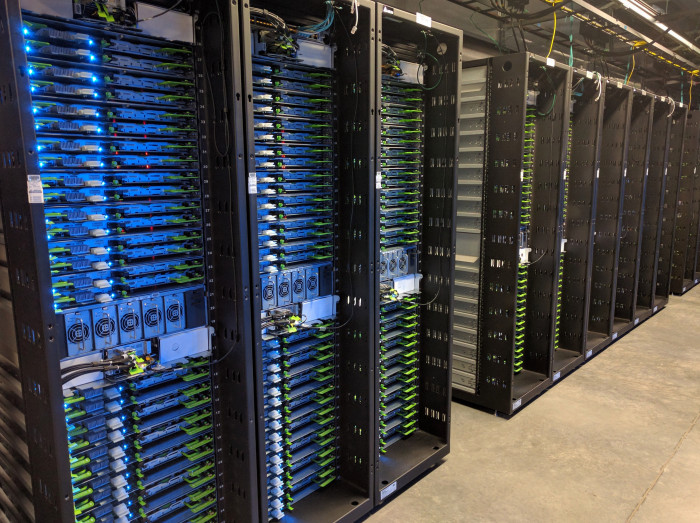
\includegraphics[width = 1.0\linewidth]{img/data_center}
	 \caption{Fragment centrum obliczeniowego \\
              Źródło: \cite{lardinois2016}}
	 \label{fig:data_center}
\end{figure}

Duża liczba danych niesie ze sobą zarówno wyzwania, jak i korzyści.
W ostatnich latach ukuło się w języku angielskim pojęcie \textit{Big Data}, które definiujemy jako duże zbiory danych zarówno ze zbiorów tradycyjnych jak i cyfrowych, które są źródłem dla nowych odkryć i analiz. \cite{Arthur2013}.
Przetwarzanie i analiza owych zbiorów danych jest skomplikowana i czasochłonna dla człowieka, dlatego z pomocą przychodzą algorytmy z dziedziny sztucznej inteligencji, a konkretnie ich podzbiór związany z uczeniem maszynowym \textit{Machine learning}, zdefiniowany dalej w rozdziale \ref{chap:teoria}.
Typowymi zastosowaniem tego typu algorytmów jest filtr antyspamowy, które klasyfikuje wiadomości jako spam na podstawie dużego zbioru wiadomości oznaczonych jako spam lub nie.
Innym popularnym zastosowaniem są systemy rekomendacji - za przykład niech posłuży system w odtwarzaczu \textit{Spotify}, który na podstawie słuchanej przez użytkownika muzyki dobiera dla niego propozycje, które również mogą mu się spodobać, ze względu na podobieństwo.
Przykładowe rekomendacje przedstawiono na rys. \ref{fig:recommendations}.

\begin{figure}[h!tb]
	 \centering
	 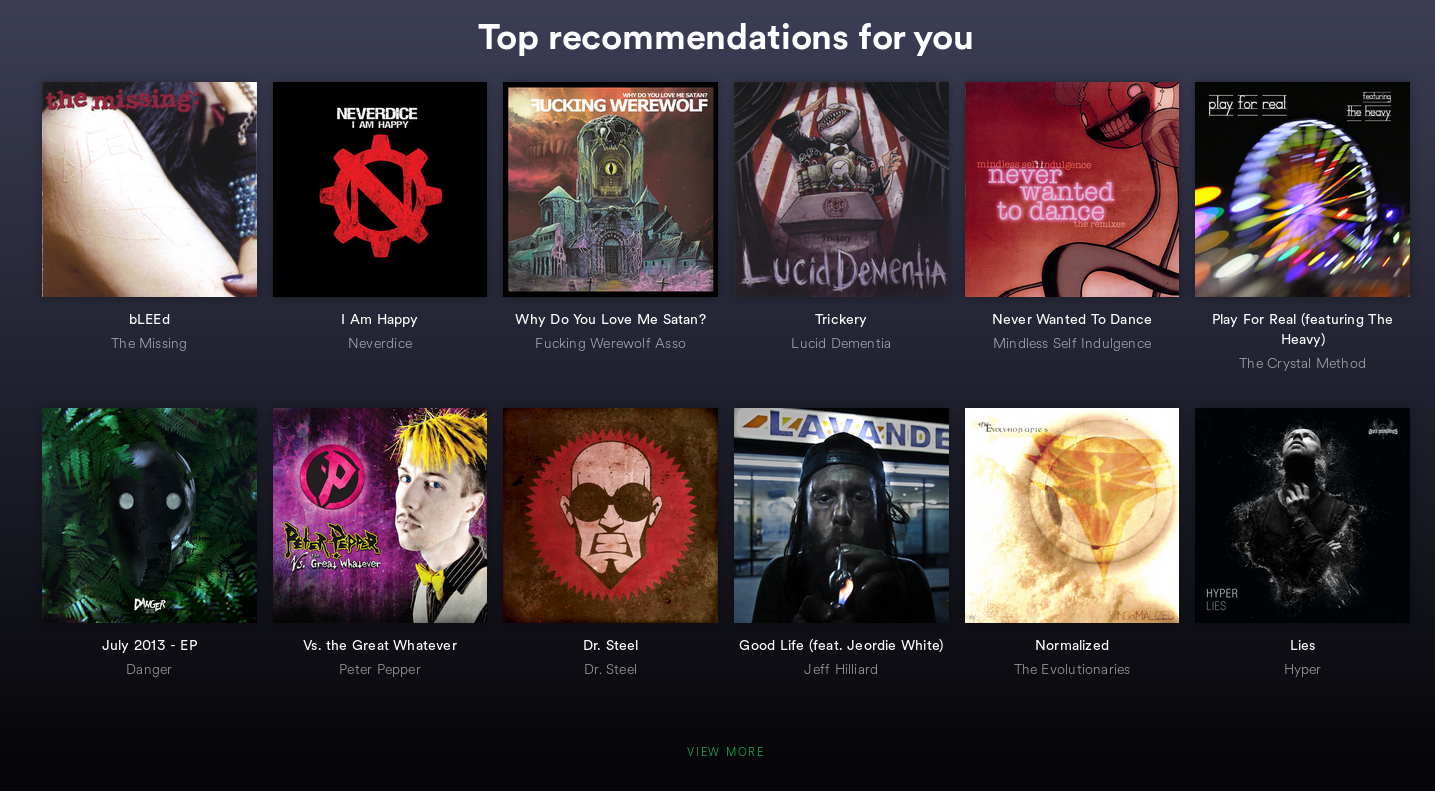
\includegraphics[width = 1.0\linewidth]{img/recommendations}
	 \caption{Rekomendowana przez algorytmy uczenia maszynowego muzyka w serwisie \textit{Spotify} \\
              Źródło: praca własna}
	 \label{fig:recommendations}
\end{figure}

Rozwiązania tego typu stosuje wiele innych popularnych serwisów multimedialnych, między innymi \textit{YouTube}, \textit{Netflix}.
Algorytmy tego typu, co zostanie przybliżone w rozdziale \ref{chap:teoria}, uczą się na podstawie podanych im danych, każdy jednak taki algorytm (np. sieci neuronowe), opisać można przez kilka parametrów.
Parametry owe można dobierać w sposób arbitralny, można jednak również do wyznaczania ich optymalnych nastaw zaprząc inny algorytm (należący również klasy algorytmów SI lub nie), np. algorytm genetyczny, algorytmy roju itd..
Inspiracją do przeprowadzenia badań w tym kierunku były zajęcia laboratoryjne z przedmiotu Sztuczna Inteligencja w Automatyce na studiach inżynierskich na kierunku Automatyka i Robotyka na wydziale Elektroniki, Telekomunikacji i Informatyki Politechniki Gdańskiej.
Jedno z zadań laboratoryjnych polegało na znalezieniu optymalnych parametrów sieci neuronowej, tak aby wynikowa sieć dobrze aproksymowała zadaną funkcję.
Korzystając z pewnej wiedzy na temat samych sieci neuronowych oraz dobierania liczby neuronów, rodzaju funkcji aktywacji, liczby warstw metodą prób i błędów ostatecznie dochodziło się do zadowalającego rozwiązania.
W tym miejscu pojawiła się idea, aby nie robić tego ręcznie, a użyć innego algorytmu.
Stąd wysunąć można główną tezę tej pracy - że możliwa jest optymalizacja owych parametrów za pomocą algorytmu genetycznego.
Dodatkowo, w związku z tym, że pełne uczenie większych sieci dla bardziej skomplikowanych problemów jak klasyfikacja obrazów jest czasochłonne, poszukiwano sposobu na skrócenie owego czasu.

Poprzez analogię do świata ludzi, gdzie można dla wielu przypadków zaobserwować prawidłowość, że mądre dzieci szybko się uczą i ostatecznie dochodzą do lepszych wyników jako dorośli, niż dzieci mniej rozgarnięte, wysnuto dodatkową tezę, mianowicie, że istnieje związek pomiędzy wynikami danej sieci neuronowej po uczeniu przez jedną epokę a jej ostateczną skutecznością po uczeniu pełnym.
Dalej przedstawiony zostanie przegląd stanu wiedzy w rozdziale \ref{chap:teoria}, zostanie opisany system, który powstał w celu udowodnienia owych tez w rozdziale \ref{chap:system_description} oraz omówione zostaną wyniki badań w rozdziale \ref{chap:tests}.
Wszystko zostanie podsumowane w rozdziale \ref{chap:summary}.

\chapter{Przegląd stanu wiedzy}\label{chap:teoria}
\section{Uczenie maszynowe}\label{machine_learning}
Mówi się, że program komputerowy uczy się z doświadczenia (\textit{experience}) E w związku z pewną klasą zadań (\textit{tasks}) T oraz miarą wydajności (\textit{performance measure}) P jeżeli jego osiągi w zadaniach w T, jak mierzone przez P, ulegają polepszeniu z doświadczeniem E. \cite{mitchell1997machine}
W przypadku pojedynczej konwolucyjnej sieci neuronowej (opisanej bliżej w \ref{sec:cnn}):
\begin{itemize}
	\item jako doświadczenie $E_{CN}$ możemy zdefiniować przetwarzanie obrazów wraz z ich etykietami klas
	\item zadaniem $T_{CN}$ nazwiemy klasyfikację obrazów
	\item miarą jakości $P_{CN}$ będzie stosunek liczby poprawnie zaklasyfikowanych zdjęć ze zbioru testowego do wielkości zbioru testowego
\end{itemize}
W przypadku algorytmu genetycznego (opisanego w \ref{sec:ag}) poszukującego optymalnej struktury sieci neurnowej:
\begin{itemize}
	\item doświadczeniem $E_{GA}$ będzie tworzenie i testowanie nowych sieci neruonowych
	\item zadanie $T_{GA}$ to poszukiwanie optymalnej w sensie $P_{CN}$ struktury (parametrów) sieci neuronowej
	\item miarą jakości $P_{GA}$ będzie miara jakośći najlepszego wygenerowanego przez algorytm osobnika
\end{itemize}
Zastosowanie jednego algorytmu z dziedziny uczenia maszynowego do poprawy procesu uczenia się innego algorytmu tej samej klasy ma ścisły związek z pojęciem metauczenia.
\section{Metauczenie}
\begin{enumerate}
	\item System metauczący się (\textit{A metalearning system}) musi zawierać podsystem uczący się, który przystosowuje się z doświadczeniem.
	\item Doświadczenie jest zdobywane poprzez wykorzystywanie metawiedzy wydobytej
	\begin{enumerate}[a)]
		\item z poprzedniego epizodu uczenia na pojedynczym zbiorze danych, i/lub
		\item z innych dziedzin lub problemów.
	\end{enumerate}
\end{enumerate}
Dodatkowo, często używanym pojęciem w metauczeniu jest pojęcie tendencyjnośći (\textit{bias}), które w tym kontekście odnosi się do zbioru założeń wpływająych na wybór hipotez opisujących dane. \cite{Lemke2015}
Hipoteza w tym kontekście oznacza funkcję predykcyjną (\textit{predictive function}) powstałą w wyniku zastosowania tradycyjnego uczenia (np. konwolucyjnej sieci neuronowej) pewnymi danymi, a wpływ na jej kształt mają ustalone założenia zaszyte w strukturze uczonego algorytmu. \cite[s.2]{Brazdil2009}
Autorzy w \cite{Brazdil2009} wyróżniają:
\begin{itemize}
	\item tendencyjność deklaratywną (\textit{declarative bias}) - specyfikuje ona reprezentację przestrzeni hipotez, np. przedstawianie hiptoez korzystając wyłącznie z sieci neuronowych
	\item tendencyjność proceduralną (\textit{procedural bias}) - wpływa na szeregowanie hipotez, np. preferowanie hipotez o krótszym czasie wykonania (\textit{runtime})
\end{itemize}
Zgodnie z tą teorią, w tradycyjnym uczeniu tendencyjność jest stała, podczas gdy metauczenie stara się ją dobierać dynamicznie. \cite{Lemke2015}
W kontekście projektowanego systemu automatycznie dobierającego parametry konwolucyjnej sieci neuronowej, spełnia ona założenia sprecyzowane w pierwszej części definicji, tj.
\begin{itemize}
	\item Istnieje uczący się podsystem (konwolucyjna sieć neurnowa)
	\item Struktura najlepszego osobnika ulega zmanie (przystosowuje się z doświadczeniem)
	\item Metawiedza jest wydobywana z poprzednich epizodów uczenia (jako wartość funkcji przystosowania konkretnej struktury)
\end{itemize}
W odniesieniu do tendencyjności deklaratywnej - przestrzeń poszukiwań (najlepszego algorytmu do klasyfikacji obrazów) została zawężona wyłącznie do konwolucyjnych sieci neruonowych, jednakże sieci o różnych strukturach będą produkować różne hipotezy.
Poszukiwanie najlepszego algorytmu do klasyfikacji obrazów na zbiorze CIFAR-10 nie jest tematem tej pracy - jest nią próba znalezienia optymalnej struktury dla konkretnego algorytmu.
W przypadku tak zawężonej przestrzeni poszukwiań dalej możemy preferować jedne generowane hipotezy od drugich, co można regulować odpowiednio modyfikując funkcję przystosowania, np. uwzględniając karę za komplikację uzyskanej struktury (np. wynikowa ilość aktywnych warstw konwolucyjnych).
\section{Uczenie z nadzorem}\label{supervised_learning}
Zadanie uczenia maszynowego nauczenia się funkcji wiążącej wejście z wyjściem na podstawie przykładowych par wejściowo-wyjściowych nazywamy uczeniem z nadzorem. \cite{russell2010artificial}
Polega ono na wywodzeniu funkcji z oznaczonych etykietami danych treningowych składających się ze zbioru przykładów treningowych. \cite{mohri2012foundations}
Przykładowy problem, który może zostać zaklasyfikowany do uczenia z nadzorem: posiadając historyczne dane miesięczne na temat ilości pożarów w danym mieście, przewidzieć ile pożarów wybuchnie w nadchodzącym miesiącu.
W tym wypadku czas (miesiąc) jest zmienną niezależną, a liczba pożarów zmienną zależną. Ustalenie związku pomiędzy tymi wielkościami (znalezienie modelu) jest zadaniem regresji, które jest jedną z podklas uczenia z nadzorem.
Drugą klasą takich problemów jest tzw. problem klasyfikacji, w którym, zamiast wyznaczać funkcję, której zbiór wartości jest (w przybliżeniu) ciągły, identyfikujemy odwzorowane, które pozowli nam nową, nieznaną daną zakwalifikować do dykretnego zbioru klas.
Popularnym przykładem jest uczenie systemu klasyfikowania wiadomości e-mail jako spam lub nie, gdy posiadamy zbiór treningowy w postaci już opisanych jako należące do odpowiedniej klasy wiadomośći.
Podczas gdy taki klasyfikator (filtr antyspamowy) przetwarza tekst, w przypadku niniejszej pracy magisterskiej mamy do czynienia z problemem klasyfikacji obrazów.
\section{Klasyfikacja obrazów}
Klasyfikacja obrazów jest zadaniem z klasy uczenia z nadzorem, w którym poszukujemy funkcji przypisującej obrazom odpowiednie etykiety z pewnego skończonego zbioru.
Jest to jeden z podstawowych problemów przetwarzania obrazów.
Co więcej, wiele pozornie różnych zadań (takich jak detekcja obiektów, segmentacja) można zredukować do problemu klasyfikacji obrazów.
Przykładowo, model klasyfikujący obrazy przetwarza zdjęcie pokazane poniżej na rys. \ref{fig:image_classification} i przypisuje prawdopodobieństwa do czterech kategorii, $\lbrace kot, pies, kapelusz, kubek \rbrace$.
Jak pokazano na rysunku, należy pamiętać, że zdjęcia dla komputera są niczym innym jak dużą trójwymiarową tablicą liczb.
W tym przypadku zdjęcie kota jest szerokie na 2048 pikseli, wysokie na 1536 pikseli i posiada 3 kanały koloru: czerwony, zielony i niebieski (z ang. w skrócie \textit{RGB}).
Tym samym zdjęcie składa się z $2048 \times 1536 \times 3 = 9437184$ liczb.

\begin{figure}[h!tb]
	 \centering
	 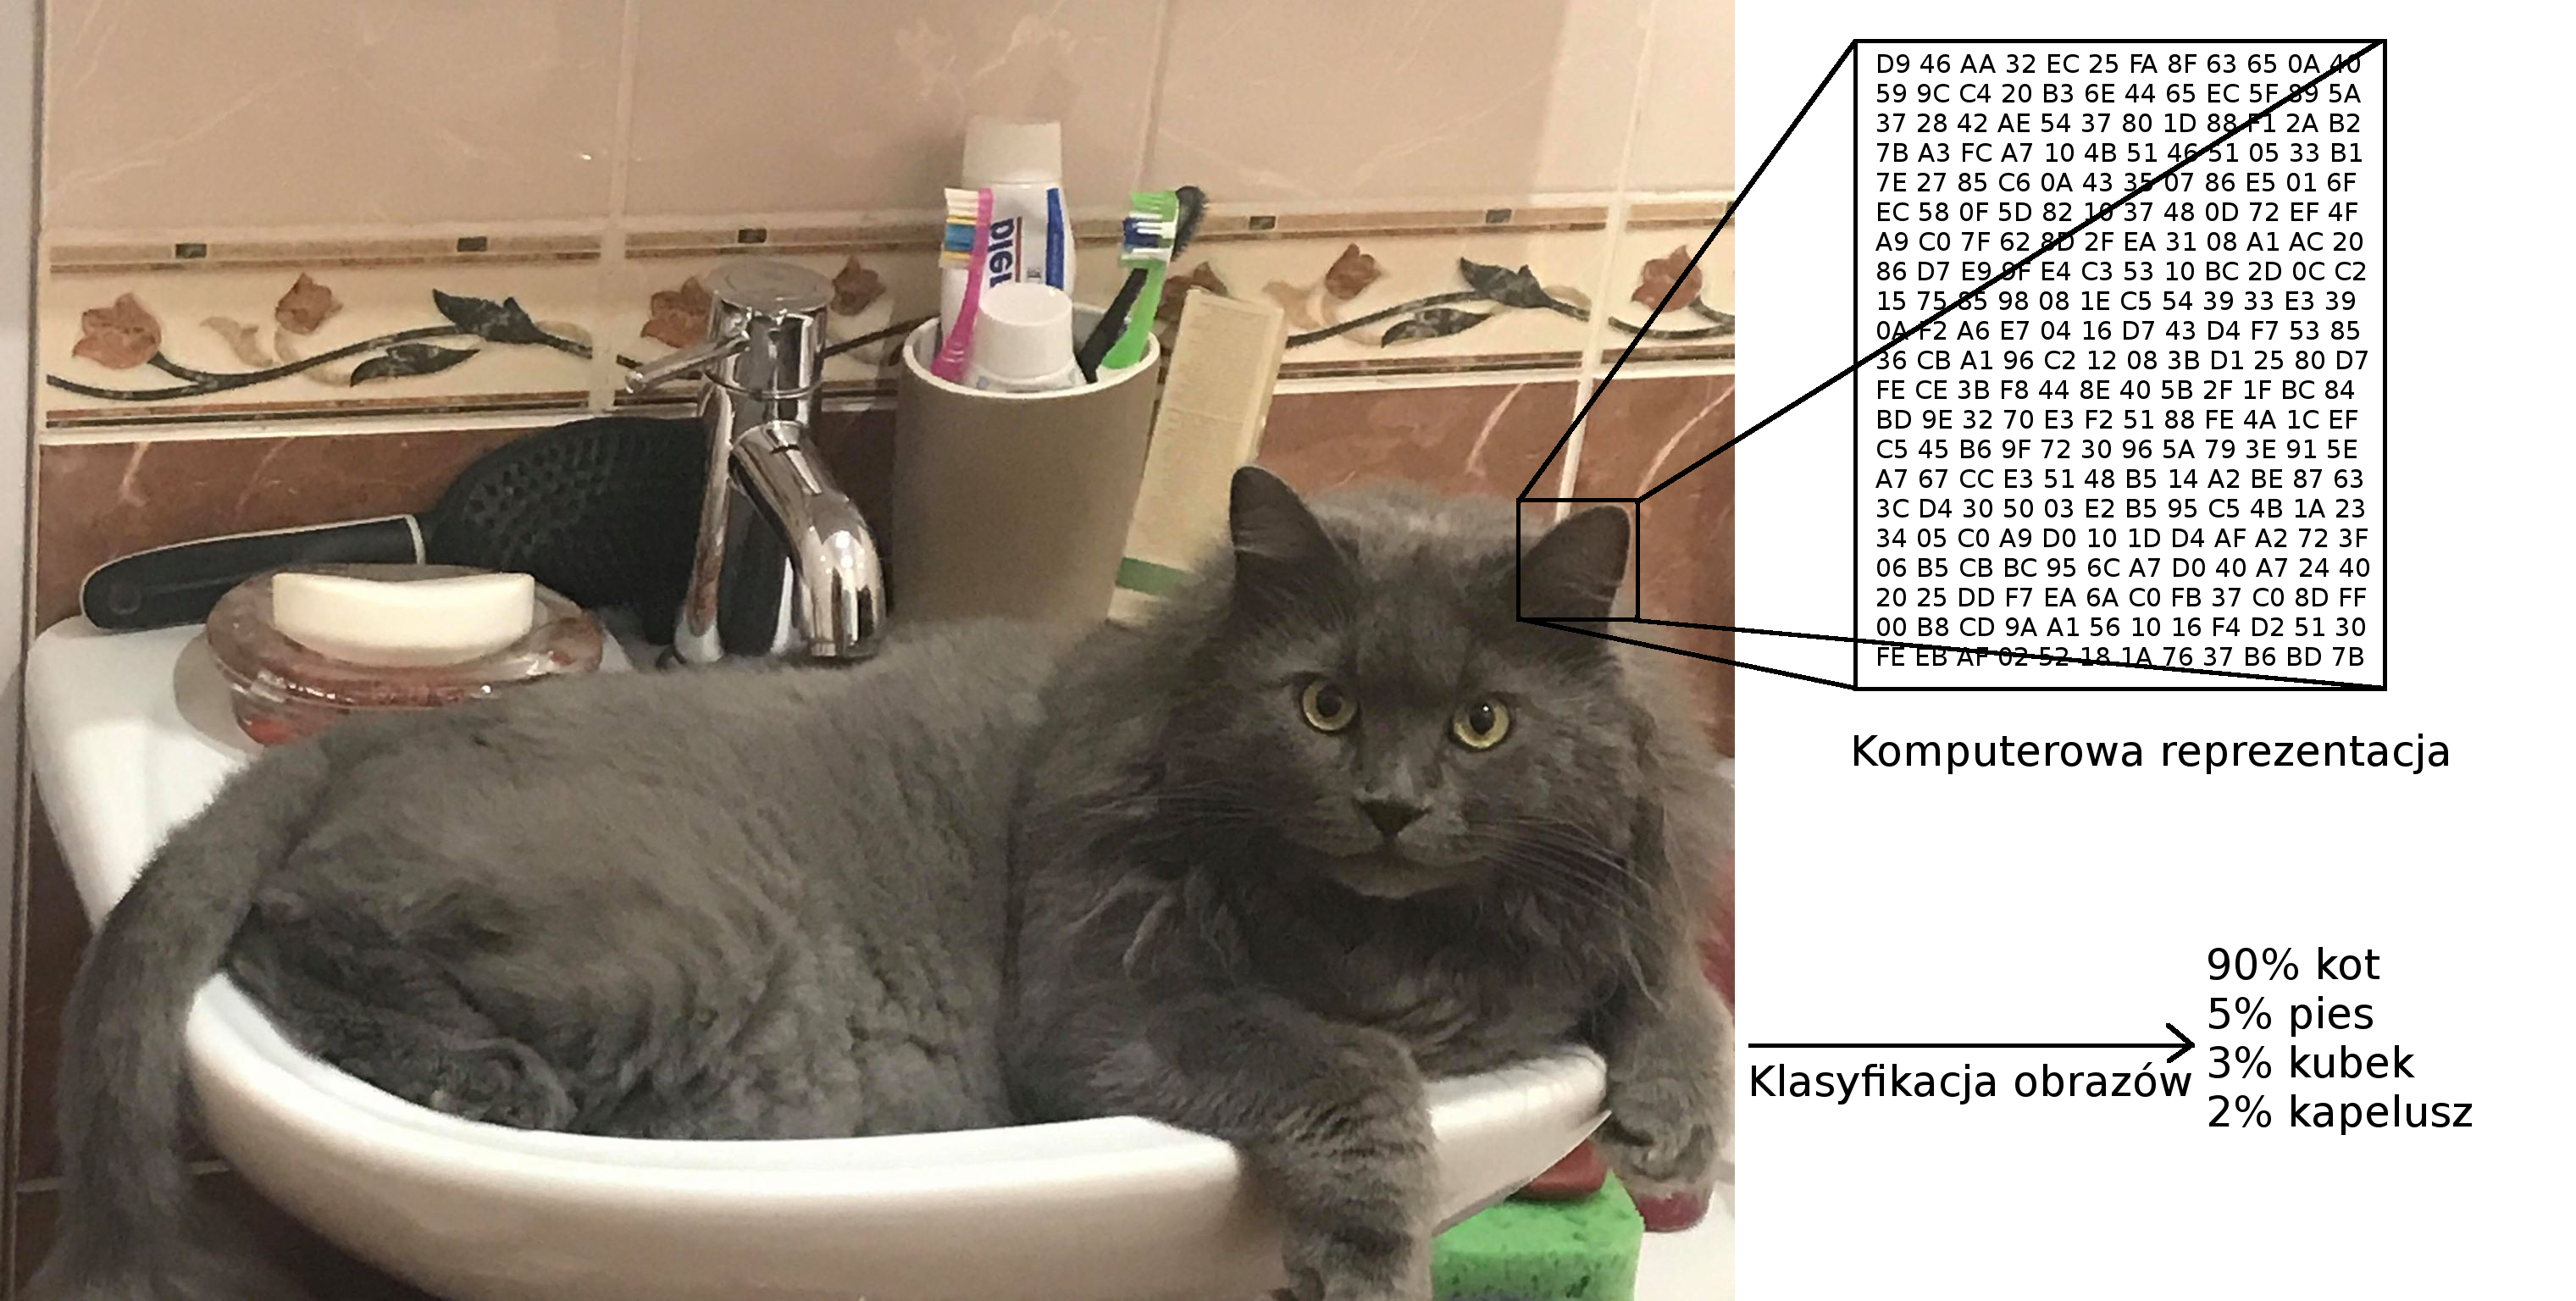
\includegraphics[width = 1.0\linewidth]{img/kot}
	 \caption{Komputerowa reprezentacja zdjęcia kota \\
              Źródło: praca własna na podstawie \cite{cs231n}}
	 \label{fig:image_classification}
\end{figure}

Zadanie klasyfikacji obrazów w tym przypadku polega na zredukowaniu tych prawie 10 milionów liczb do jednej etykiety, dla rys. \ref{fig:image_classification} będzie to ''$kot$''.
Dla człowieka rozpoznanie obiektu jest względnie proste. Z punktu widzenia algorytmu przetwarzania obrazów napotykamy kilka zasadniczych trudności, związanych z faktem, że komputer interpretuje obraz jako trójwymiarową macierz wartości jasności pikseli:
\begin{itemize}
	\item Zróżnicowanie perspektywy - ten sam obiekt może być różnie zorientowany względem kamery rejestrującej obraz
	\item Zróżnicowanie skali - obiekty jednej klasy (np. koty) często występują w różnych rozmiarach (nie tylko z punktu widzenia rozmiaru na zdjęciu, ale i w rzeczywistości)
	\item Deformacja - wiele klasyfikowanych obiektów nie jest bryłami sztywnymi i mogą być skrajnie zniekształcone
	\item Okluzja - zjawisko zasłonięcia obiektu przez inny obiekt, czasem jedynie niewielki fragment szukanego obiektu jest widoczny
	\item Warunki oświetleniowe - efekty różnego oświetlenia są bardzo wydatne na poziomie pikseli
	\item Nieład w tle - klasyfikowane obiekty mogą zlewać się z tłem, czyniąc ich identyfikację trudniejszą
	\item Zróżnicowanie wewnątrz klasy - niektóre klasy są bardzo ogólne (np. broń) i zawierają w sobie bardzo różnie wyglądające obiekty (np. miecz a karabin maszynowy).
\end{itemize}
Na rys.\ref{fig:classification_problems} przedstawiono ilustrację powyższych problemów.

\begin{figure}[h!tb]
	 \centering
	 
\includegraphics[width = 1.0\linewidth]{img/klas_problemy}
	 \caption{Problemy w klasyfikacji obrazów \\
              Źródło: praca własna na podstawie \cite{cs231n}}
	 \label{fig:classification_problems}
\end{figure}

Dobry model klasyfikujący obrazy powienien być niewrażliwy na dowolne kombinacje powyższych zakłóceń, jednocześnie pozostając wrażliwym na zróżnicowanie pomiędzy klasami.
Stworzenie algorytmu poprawnie klasyfikującego obrazy jest zadaniem nietrywialnym (w przeciwieństwie np. do ułożenia algorytmu sortującego liczby według zadanego porządku).
Jednym ze podejść, jakie można przyjąć do tego problemu, jest stworzenie algorytmu, który będzie się uczył na podstawie dużej ilości oznaczonych etykietami danych, czyli wspomniane wcześniej uczenie maszynowe (\ref{machine_learning}) i uczenie z nadzorem (\ref{supervised_learning}).
Takie rozwiązanie problemu nazywane jest również podejściem opartym na danych (\textit{data-driven approach}).
\cite{cs231n}


\section{CIFAR-10}
Przykładem zbioru danych służącego do uczenia i oceny algorytmów uczenia maszynowego w dziedzinie klasyfikacji obrazów jest zbiór CIFAR-10.
Zbiór danych CIFAR-10 składa się z 60000 kolorowych obrazków o wymiarach 32x32 pogrupowanych w 10 klas, po 6000 obrazków w każdej. Zbiór trenigowy składa się z 50000 obrazków, a testowy z 10000.

Dane zorganizowane są w pięć partii trenigowych i jedną testową, po 10000 obrazków każda. Partia testowa zawiera dokładnie po 1000 losowo wybranych obrazków z każdej klasy. Partie treningowe zawierają pozostałe obrazki w losowej kolejności, w związku z czym niektóre partie mogą zawierać więcej obrazków z jednej klasy niż pozostałych. Łącznie zawierają po 5000 obrazków z każdej klasy.

Poniżej, na rysunku \ref{fig:sample_data} przedstawiono wszystkie klasy wraz z 10 losowymi obrazkami dla każdej z nich.
\begin{figure}[h!tb]
	 \centering
	 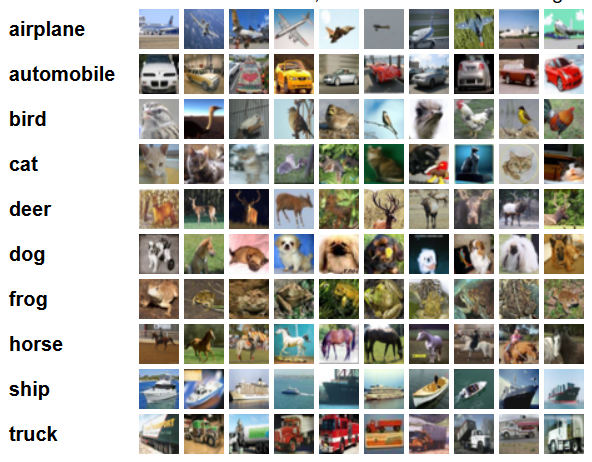
\includegraphics[width = 1.0\linewidth]{img/sample_images}
	 \caption{Przykładowe obrazki ze zbioru CIFAR-10 \\
              Źródło: https://www.cs.toronto.edu/\textasciitilde kriz/cifar.html}
	 \label{fig:sample_data}
\end{figure}

Każda z klas wyklucza się wzajemnie. Klasy ''samochód'' (\textit{automobile}) i ''ciężarówka'' (\textit{truck}) nie posiadają części wspólnej. ''Samochód'' zawiera sedany, SUVy i inne tego typu samochody. ''Ciężarówka'' zaiwera tylko duże ciężarówki. Żadna z nich nie zawiera pojazdów typu pickup.

Poniżej opisano organizację tego zbioru danych w wersji dla języka Python.

Archiwum zawiera pliki data\_batch1, data\_batch2 data\_batch5, jak również test\_batch. Każdy z tych plików jest poddaną serializacji wersją obiektu Pythonowego wytworzonego za pomocą cPickle. Poniżej, na listingu \ref{lst:read_data} przedstawiono procedurę odczytującą te pliki i zwracającą słownik dla Pythona w wersji 2:

\begin{lstlisting}[caption={Procedura ładowania zbioru danych},label={lst:read_data},language=Python,captionpos=b,frame=single]
def unpickle(file):
    import cPickle
    with open(file, 'rb') as fo:
        dict = cPickle.load(fo)
    return dict
\end{lstlisting}

    Załadowane w ten sposób, każdy z plików z partiami zawiera następujące elementy:
\begin{itemize}
\item \textit{data} - macierz \textit{numpy} typu \textit{uint8} o wymiarach 10000x3072. Każdy rząd macierzy przechowuje kolorowy obrazek o wymiarach 32x32. Pierwsze 1024 pozycji zawiera wartości pikseli dla kanału czerwononego, kolejne 1024 dla zielonego, a ostatnie dla niebieskiego. Zdjęcia przechowywane są rzędami w kolejności od góry do dołu, tj. pierwsze 32 elementy macierzy opisują wartości kanału czerwonogo dla pierwszego rzędu pikseli obrazka.
\item \textit{labels} - lista 10000 liczb w przedziale 0-9. Liczba pod indeksem i oznacza etykietę z klasą dla i-tego obrazka w macierzy data.
\end{itemize}

Zbiór danych zawiera również plik batches.meta, który również zawiera obiekt typu słownik dla języka Python. Zawiera on następujące elementy:
\begin{itemize}
\item \textit{label\_names} - 10 elementowa lista która nadaje czytelne dla człowieka nazwy liczbowym etykietom w liście \textit{labels} opisanej powyżej. Na przykład, label\_names[0] == ''airplane'', label\_names[1] == ''automobile'', itd. \cite{Krizhevsky09learningmultiple}
\end{itemize}

Wśród kilku podejść, które mogą nam posłużyć do rozwiązania tego problemu, wyróżnić możemy algorytm k najbliższych sąsiadów (\textit{k - Nearest Neighbour Classifier}), klasyfikatory liniowe, sieci neuronowe.

\section{K najbliższych sąsiadów}\label{sec:knear}

Dla zbioru CIFAR-10 mamy $50000$ obrazków oznaczonych etykietami i $10000$ obrazów, które chcemy zaklasyfikować.
Każdy obrazek o wymiarach $32 \times 32 \times 3$ możemy przedstawić jako wektor o wymiarach $3072 \times 1$.
Oznacza to, że każdy z nich możemy interpretować jako punkt w przestrzeni $3072$-wymiarowej.
Najprotszym sposobem w jaki możemy klasyfikować nowe dane jest badanie ich położenia w owej przestrzeni.
Zakładając, że obrazki jednej klasy będą grupować się w klastry, każdy kolejny punkt znajdujący się blisko chmury punktów reprezentującej daną klasę z wysokim prawdopoboieństwem również będzie przynależał do tej klasy.
Przykładowo, rozważmy sytuację jak na rys. \ref{fig:knearest} dla klasyfikacji dwuwymiarowych punktów. Punkt albo przynależy do klasy 'niebieski okrąg', albo 'czerwony krzyżyk'. Rozważamy punkt, który oznaczony jest zielonym krzyżykiem.

\begin{figure}[h!tb]
	 \centering
	 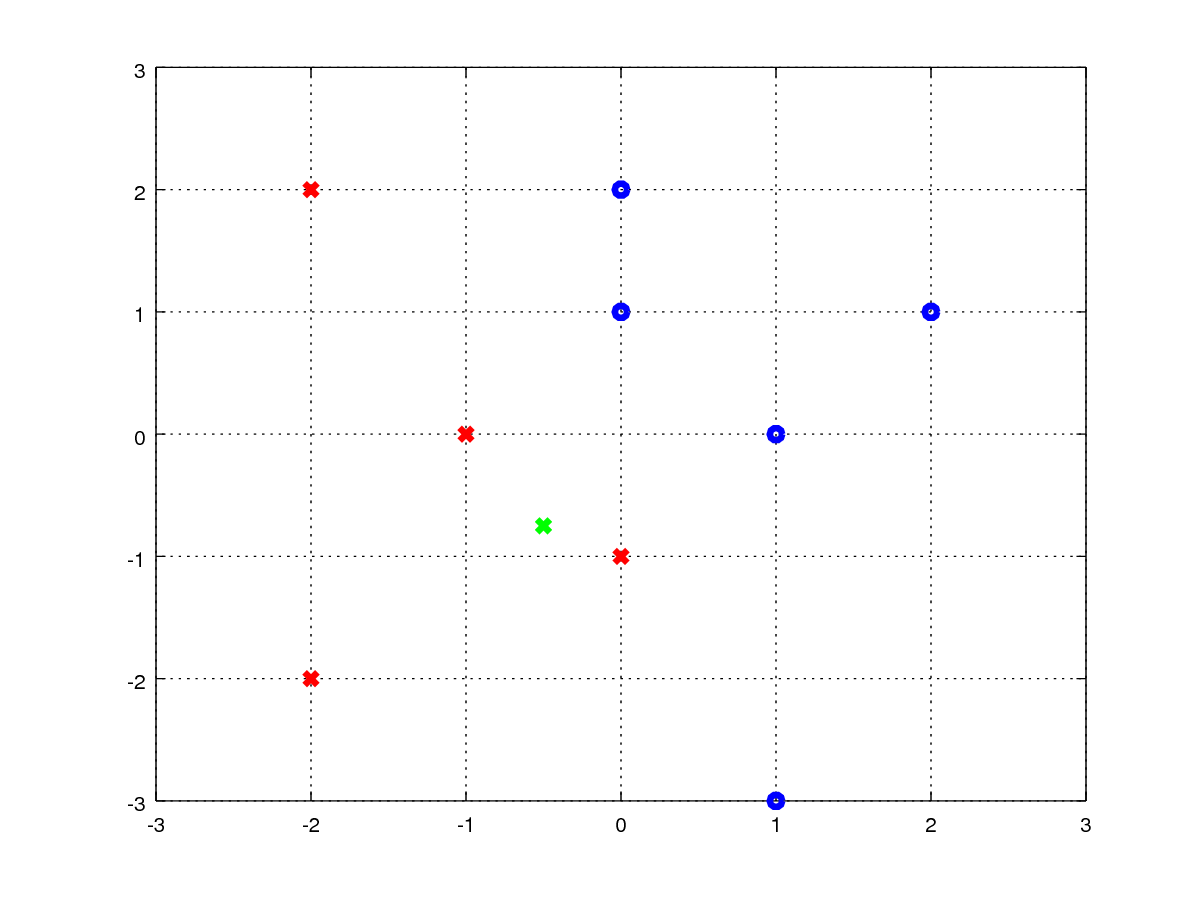
\includegraphics[width = 1.0\linewidth]{img/knear}
	 \caption{Ilustracja działania algorytmu k najbliższych sąsiadów w dwóch wymiarach \\
              Źródło: praca własna}
	 \label{fig:knearest}
\end{figure}

Dla najprostszego przypadku $k=1$ badamy odległości (w tym przypadku użwyając normy $l^2$) pomiędzy interesującym nas punktem a wszystkimi danymi ze zbioru treningowego i przyjmujemy, że badany punkt będzie przynależał do tej samej klasy, do której przynależy jej najbliższy sąsiad.
W przypadku rys. \ref{fig:knearest} badany zielony punkt znajduje się najbliżej czerwonego krzyżyka w punkcie $(0,-1)$, zatem przypisujemy go do tej samej klasy.
Dla większych wartości k rozważamy więcej najbliższych sąsiadów i przypisujemy rozważany punkt do tej klasy, do której należy większość najbliższych punktów.

Podejście to, mimo iż intuicyjne i proste w implementacji, nie rozwiązuje dobrze problemu klasyfikacji, osiągając skuteczność $39.6\%$ dla $k = 1$ dla zbioru CIFAR-10.
Jest to lepiej niż losowe przydielanie do klas (które dla 10 klas ma skuteczność $10\%$), ale wciąż dalekie od skuteczności człowieka.

Jednym z problemów podejścia k najbliższych sąsiadów jest kosztowne testowanie nowych punktów.
Dla każdego nowego punktu wymaga ono policzenia odległości od 50000 punktów w przestrzeni 3072-wymiarowej oraz posortowania wg. obliczonej odległości, co jest dość kosztowną operacją.

Kolejnym problemem w przypadku przetwarzania obrazów jest klasyfikowanie wyłącznie na podstawie dominujących w obrazie wartości kolorów.
Na przykład, zarówno w przypadku klasy ''samolot'' jak i w przypadku klasy ''statek'' często występującym w tle kolorem będzie niebieski, gdyż niebieskie jest zarówno niebo i woda.
Tak duże podobieństwo może prowadzić do błędnej klasyfikacji w przypadku tych dwóch klas. \cite{cs231n}

\section{Klasyfikator liniowy}

Innym podejściem, jakie można przyjąć do klasyfikacji obrazów, jest stworzenie liniowego odwzorowania pomiędzy pikselową reprezentacją obrazu a stopniem przynależności danego obrazu do poszczególnych klas.
Oznaczając dane treningowe przez $x_i \in R^D$, każde powiązane z etykietą $y_i$.
W tym przypadku $i = 1 ... N$ i $y_i \in 1 ... K$, tj. zbiór uczący składa się z $N$ przykładów (każdy D-wymiarowy) i K rozróżnialnych kategorii.
Przykładowo, dla zbioru CIFAR-10 zbiór treningowy ma rozmiar $N = 50000$, każdy po $32 \times 32 \times 3 = 3072$ pikseli i $K = 10$, poniważ rozróżniamy pomiędzy 10 klasami (pies, kot, samochód itd.).
Zdefiniujemy funkcję oceny (\textit{score function}) $f : R^D \mapsto R^K$, która odwzorowuje wartości pikseli do oceny przynależności do danej klasy.
Zatem liniowy klasyfikator zdefiniować jako następujące liniowe odwzorowanie:
\begin{equation}\label{eqn:lc}
f(x_i,W,b) = Wx_i + b
\end{equation}
We wzorze \ref{eqn:lc} zakładamy, że obrazek $x_i$ zawiera wszystkie wartości swoich pikseli w wektorze o wymiarach $[D \times 1]$.
Macierz $W$ (o wymiarach $[K \times D$]) oraz wektor $b$ (o wymiarach [$K \times 1$]) są parametrami funkcji.
W zbiorze CIFAR-10 $x_i$ zawiera wszystkie piksele $i$-tego obrazka spłaszczone do jednej [$3072 \times 1$] kolumny, $W$ ma wymiar [$10 \times 3072$] a $b$ [$10 \times 1$], zatem 3072 liczby są wejściem dla funkcji, a wyjść jest 10 (oceny klas).
Parametry wewnątrz $W$ nazywane są również wagami, a wektor $b$ nazywany jest wektorem przesunięcia (\textit{bias vector}), ponieważ ma wpływ na wyjściowe ocenu bez wchodzenia w interakcję z danymi $x_i$. \cite{cs231n}

Jak już wspominano, obrazki mogą być rozumiane jako punkty w 3072 wymiarowej przestrzeni.
Pojedynczy liniowy klasyfikator możemy interpretować jako hiperpłaszczyznę separującą punkty w tej przestrzeni.
Możemy wyobrazić sobie ściśnięcie wszystkich punktów do dwóch wymiarów jak na rys. \ref{fig:cartoon_class}, wtedy hiperpłaszczyny sprowadzają się do prostych.

\begin{figure}[h!tb]
	 \centering
	 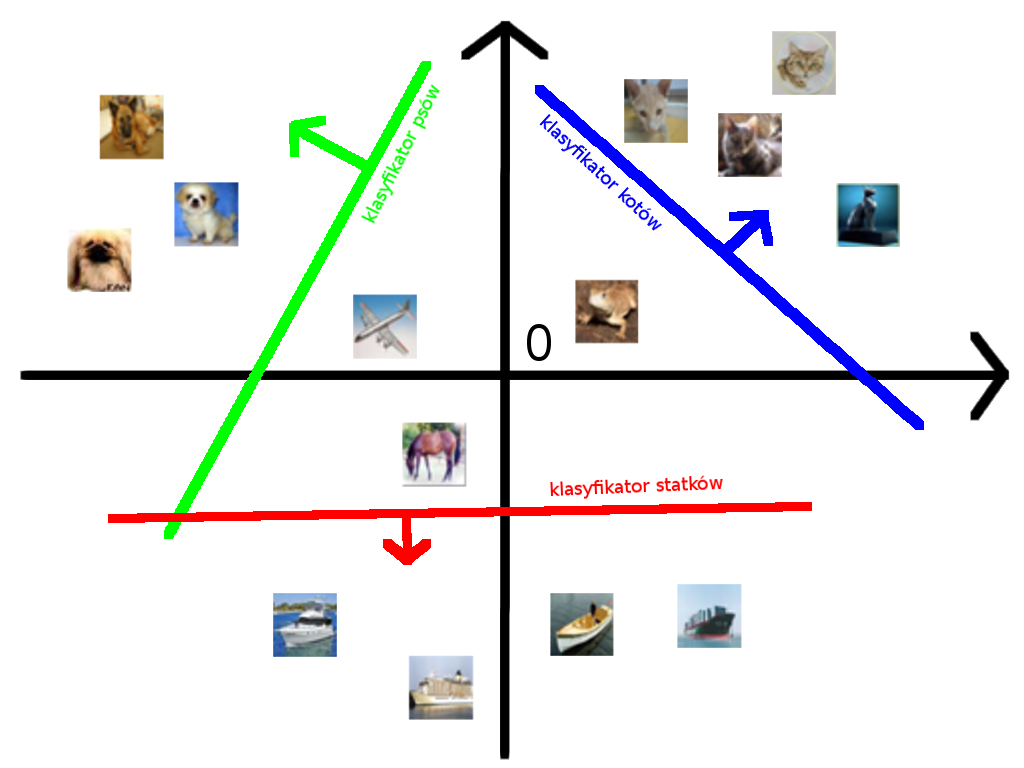
\includegraphics[width = 0.75\linewidth]{img/klas_cartoon}
	 \caption{Schematyczna wizualizacja działania klasyfikatorów liniowych \\
              Źródło: praca własna na podstawie \cite{cs231n}}
	 \label{fig:cartoon_class}
\end{figure}

Przy klasyfikatorze liniowym warto zauważyć kilka faktów:
\begin{itemize}
	\item Pojedyncze mnożenie macierzowe $Wx_i$ w efekcie wyznacza oceny dla 10 różnnych klasyfikatorów jednocześnie (jeden na klasę), gdzie każdy klasyfikator to rząd macierzy W i jednej prostej separującej na rys. \ref{fig:cartoon_class}
	\item Dane wejściowe $(x_i,y_i)$ są ustalone, a kontrolujemy parametry $W,b$. Naszym celem będzie ustawienie tych parametrów w taki sposób, by wynikowe oceny zgadzały się z prawdziwymi przynależnościami do klas na całym zbiorze treningowym.
	\item Zaletą tego podejścia jest możliwość odrzucenia (nie przechowywania w pamięci) zbioru treningowego po nauczeniu się parametrów $W,b$. Dzieje się tak, ponieważ nowe punkty do klasyfikacji klasyfikujemy przy pomocy ocen uzyskanych z już nauczonej funkcji.
	\item Klasyfikowanie obrazów testowych sprowadza się do pojedynczego mnożenia macierzowego i dodawania, które jest szybsze od porównywania do wszystkich obrazków ze zbioru treningowego (jak w \ref{sec:knear}).
\end{itemize}

Przykład mapowania wartości pikseli do oceny przynależności do klas przedstawiono na rys. \ref{fig:lin_class}
\begin{figure}[h!tb]
	 \centering
	 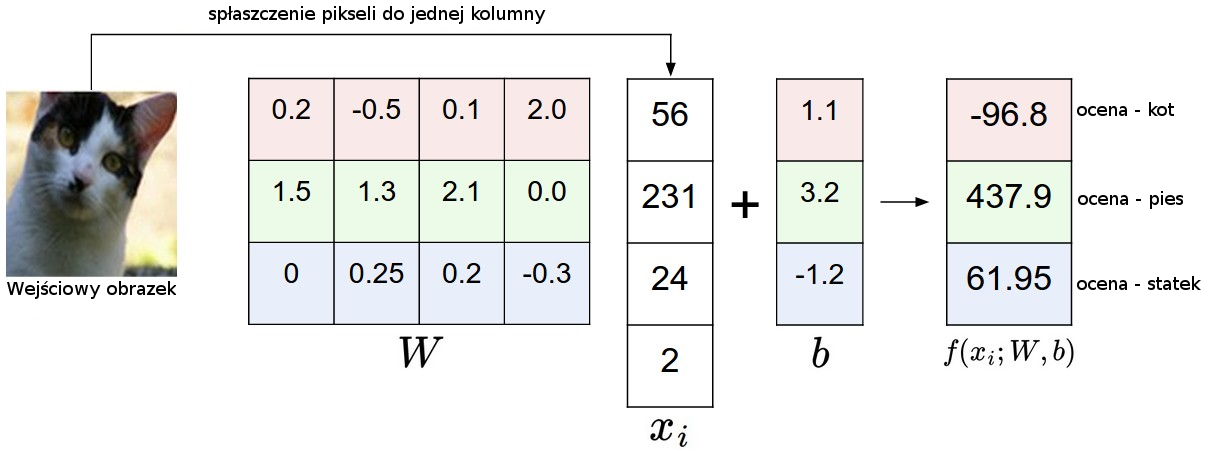
\includegraphics[width = 1.0\linewidth]{img/lin_klas}
	 \caption{Mapowanie 4 monochromatycznych pikseli do 3 klas \\
              Źródło: praca własna na podstawie \cite{cs231n}}
	 \label{fig:lin_class}
\end{figure}

Jak widać na rys. \ref{fig:lin_class}, wagi w macierzy W nie są dobrze dobrane, gdyż klasyfikator przypisuje najwyższą ocenę klasie pies, podczas gdy w istocie na obrazku znajduje się kot.
Uczenie liniowego klasyfikatora będzie polegać na takim doborze wag, by błędy klasyfikacji zachodziły jak najrzadziej.
W tym celu zdefinujemy funkcję kosztów (\textit{loss function}), która będzie miarą tego jak dobrze działa dany klasyfikator.\cite{cs231n}

Funkcję kosztów dla całego zbioru danych definuje wzór \ref{eqn:total_loss}.
\begin{equation}\label{eqn:total_loss}
L =  \underbrace{ \frac{1}{N} \sum_i L_i }_\text{składowa danych} + \underbrace{ \lambda R(W) }_\text{składowa regularyzacji} \\\\
\end{equation}
gdzie $\lambda$ jest parametrem kontrolującym oddziaływanie regularyzacji przy uczeniu, $L_i$ wartością funkcji kosztu dla pojedynczego obrazka przy ustalonych wagach W (wzór \ref{eqn:single_loss_svm} lub \ref{eqn:single_loss_softmax}).
Składowa regularyzacji penalizuje duże wagi w macierzy $W$ i w tym przypadku będzie definiowana jako norma $l^2$ dla tej macierzy, zgodnie ze wzorem \ref{eqn:regularization}.

\begin{equation}\label{eqn:regularization}
R(W) = \sum_k\sum_l W_{k,l}^2
\end{equation}

Wprowadzenie tej składowej do funkcji kosztu pozwala uniknąć niejednoznaczności rozwiązania, gdzie dowolna macierz $W$ przeskalowana o współczynnik $\alpha \in R^+$ jest równie dobrym rozwiązaniem.
W ten sposób prefeorwane będą rozwiązania o o mniejszych wartościach współczynników.
Co więcej, okazuje się, że przy takim podejściu uzyskujemy lepiej generalizujące i bardziej odporne na nadmierne dopasowanie (\textit{overfitting}) klasyfikatory.
Wynika to z faktu, że żaden z wejściowych wymiarów nie może mieć dużego wpływu na końcowy wynik.
Dla przykładu, dla wektora danych $x = [1,1,1,1]$ i dwóch wektorów wagowych $w_1 = [1,0,0,0]$ i $w_2 = [0.25,0.25,0.25,0.25]$ wynik mnożenia (wartość funkcji oceny) $w_1^Tx = w_2^Tx = 1$.
Jednakże wprowadzenie kary $l^2$ do funkcji kosztu powoduje, że preferowany będzie wektor $w_2$, gdyż $||w_2|| < ||w_1||$, a naszym celem jest minimalizacja funkcji kosztów.
Widać zatem, że preferowane będą wektory wagowe o bardziej rozłożonych współczynnikach.

Składowa danych ze wzoru \ref{eqn:total_loss} jest funkcją kosztu dla pojedynczego obrazka uśrednioną po wszystkich danych treningowych.
Dla $i$-tego punktu treningowego możemy zdefinować wiele różnych funkcji kosztu.
Dla klasyfikatora typu wieloklasowa maszyna wektorów nośnych (\textit{Multiclass SVM}) będzie to koszt ''zawiasowy'' (\textit{hinge loss}, wzór \ref{eqn:single_loss_svm}), natomiast dla klasyfikatora typu \textit{Softmax} koszt entropii krzyżowej (\textit{cross-entropy loss}, przedstawiony na wzorze \ref{eqn:single_loss_softmax}).
\begin{equation}\label{eqn:single_loss_svm}
L_i = \sum_{j\neq y_i} \max(0, s_j - s_{y_i} + \Delta)
\end{equation}
gdzie $s_j = f(x_i, W)_j$ to $j$-ty element wektora ocen klas, $s_{y_i}$ jest oceną uzyskaną przez prawdziwą klasę, a $\Delta$ jest marigniesem, który chcemy utrzymać pomiędzy wartością oceny klasy prawdziwej a wartościami ocen klas niepoprawnych.

\begin{equation}\label{eqn:single_loss_softmax}
L_i = -\log\left(\frac{e^{s_{y_i}}}{ \sum_j e^{s_j} }\right) \hspace{0.5in} \text{lub równoważnie} \hspace{0.5in} L_i = -s_{y_i} + \log\sum_j e^{s_j}
\end{equation}
gdzie $s_j$ jak wyżej oznacza $j$-ty element wektora ocen klas $s$, tutaj interpretowany jako nieznormalizowany logarytm prawdopodobieństwa przynależności do danej klasy.

Możemy teraz znaleźć taką macierz wagową $W$, która minimalizuje wartość przyjętej funkcji kosztu, tym samym maksymalizując poprawność działania klasyfikatora.
Jest to problem optymalizacji, który rozwiązujemy najczęściej przy pomocy gradientowych metod optymalizacji, np. metody najszybszego spadku. \cite{cs231n}

Powodem, dla którego tyle miejsca poświęcono liniowemu klasyfikatorowi i pojęciami z nim związanymi jest fakt, że wszystkie te pojęcia mają również zastosowanie przy sieciach neuronowych.

\section{Sieci Neruonowe}\label{sec:nn}

\begin{figure}[h!tb]
	 \centering
	 \includegraphics[width = 1.0\linewidth]{img/neuron}
	 \caption{Pojedynczy 3-wejściowy neuron \\
              Źródło: praca własna na podstawie \cite{cs231n,zuradabarskijedruch1996}}
	 \label{fig:neuron}
\end{figure}

Zarówno zwierzęta, jak i ludzie lepiej radzą sobie z rozpoznawaniem obrazów niż współczesne komputery.
Sieci neuronowe dlatego wzbudzają zainteresowanie, że możemy za ich pomocą częściowo naśladować ludzki mózg.
Informacja w takich sieciach przetwarzana jest przez dużą ilość węzłów obliczeniowych oraz połączeń między nimi.
Skoordynowane jednoski jednocześnie dokonują przetwarzania wszystkich lub większości sygnałów i danych wejściowych.
Działanie sztucznych sieci neuronowych możemy porównać do rozproszonych systemów obliczeniowych.
Elementarną jednostkę wykonującą obliczenia w takiej sieci nazywamy neuronem.
Pojedynczy neuron dokonuje sumowania i nieliniowego przetwarzania sygnałów.
Nierzadko możemy je przyrównać do elementów działających progowo, aktywujących się w momencie przekroczenia pewnego zadanego progu przez sumę sygnałów na wejściu.
Często neurony organizowane są w regularne struktury, zwykle możemy w owych strukturach wyróżnić poszczególne warstwy.
Możliwe jest występowanie połączeń zwrotnych pomiędzy neuronami tej samej warstwy lub z różnych warstw.
Każde połączenie pomiędzy neuronami charakteryzowane jest przez siłę jego oddziaływania zwaną również wagą. \cite{zuradabarskijedruch1996}

Schematycznie pojedynczy neuron możemy przedstawić jak na rys. \ref{fig:neuron}

Architektura sieci jest tym co odróżnia konkretne sieci od siebie.
Na przykład sieci nie posiadające połączeń zwrotnych reagują na pobudzenie w sposób natychmiastowy i te własnie sieci będą omawiane w dalszej części pracy.
Natomiast sieci, które posiadają połączenia zwrotne, ustalają swoją odpowiedź dopiero po pewnym czasie, mają zatem swoją dynamikę określające ich zachowanie w czasie. \cite{zuradabarskijedruch1996}



\section{Konwolucyjne sieci neuronowe}\label{sec:cnn}

Konwolucyjne sieci neuronowe (\textit{Convolutional Neural Networks}) są podobne do opisanych w \ref{sec:nn} sieci neuronowych.
Tworzone są z neuronów, które posiadają swoje wagi, które zmieniają się w wyniku procesu uczenia.
Każdy z neuronów otrzymuje sygnały na wejściu, dokonuje ich sumowania, a następnie może dokonać nieliniowego odwzorowania.
Cała sieć wyraża pojedynczą, różniczkowalną funkcję odwzorowującą wartości jasności pikseli do zbioru klas.
Sieci te projektowane są z założeniem, że będą przetwarzały obrazy, stąd ich specyficzna architektura, która zostanie opisana poniżej.

Motywacją stojącą za poszukiwaniem innych architektur sieci neuronowych była bardzo szybko narastająca ilość wag do uczenia w przypadku przetwarzania obrazów za pomocą w pełni połączonych sieci neuronowych.
Biorąc dla przykładu CIFAR-10 i obrazki o wymiarach $ 32 \times 32 \times 3$ (wysokość, szerokość, 3 kanały kolorów), pojedynczy neuron znajdujący się zaraz za warstwą wejściową posiadałby 3072 + 1 wejście od stałej wartości (\textit{bias}) wag do nauczenia.
Dla tak małych obrazków liczba ta nie wydaje się być problematyczna, jednak podając na wejście obraz o wymiarach $1024 \times 768 \times 3 = 2359296$ widzimy, że już pojedynczy neuron zaczyna zajmować bardzo dużo pamięci.
Zakładając, że każda waga przechowywana jest jako liczba zmiennoprzecinkowa o podwójnej precyzji i przechowoywana w 8 bajtach, uzyskujemy $18874368$ B $= 18$MB na jeden neuron.
Tak duża liczba parametrów jest nadmiarowa i może prowadzić do nadmiernego dopasowania.

Przykładową sieć neuronową moglibyśmy zdefiniować w następujący sposób:

\cite{cs231n}

\section{Algorytm geneteyczny}\label{sec:ag}

Działanie algorytmu genetycznego można schematycznie przedstawić jak na rysunku \ref{fig:gen_schemat}

\begin{figure}[h!tb]
	 \centering
	 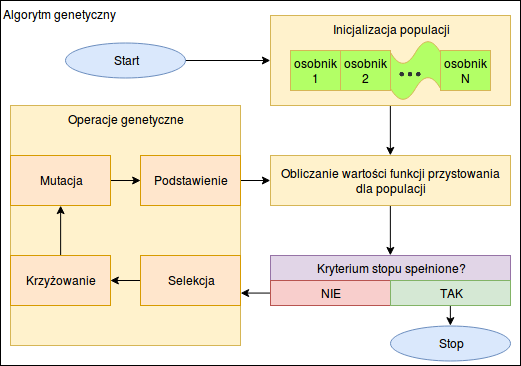
\includegraphics[width = 1.0\linewidth]{img/genetyczny_schemat}
	 \caption{Schemat działania algorytmu genetycznego \\
              Źródło: praca własna}
	 \label{fig:gen_schemat}
\end{figure}

\chapter{Opis rozwiązania}\label{chap:system_description}
W tym rozdziale następuje uściślenie problemu oraz doprecyzowanie zasad działania algorytmu genetycznego.
Również opisywany jest cały system stworzony do przeprowadzenia badań.
\section{Redukcja problemu}\label{sec:reduction}
Jak już wspomniano w rozdziale \ref{chap:teoria}, uczenie głębokich sieci neuronowych w celu klasyfikacji obrazów dla dużych danych wejściowych jest zadaniem czasochłonnym.
Jednym ze sposobów redukcji tego czasu jest stosowanie architektury konwolucyjnej (opisanej w \ref{sec:cnn}), która znacznie redukuje liczbę wag do nauczenia, a przy tym i czas obliczeń.
Nauczenie pojedynczej sieci konwolucyjnej wymaga wielu epok uczenia, najczęściej wykorzystując zrównoleglenie obliczeń na kartach graficznych, np. wykorzystując bibliotekę CUDA w połączeniu z biblioteką TensorFlow.
Osiągnięcie skuteczności klasyfikacji na poziome 86\% dla zbioru CIFAR-10 dla przykładowej sieci zajmuje ok. $t_{cnn} = 3$ godzin dla typowej karty graficznej \textit{Nvidia Geforce GTX850M}. \cite{tensorflow2015-whitepaper}

W przypadku algorytmu genetycznego, jedna konwolucyjna sieć neuronowa jest jednym osobnikiem charakteryzowanym przez jego fenotyp, opisany w \ref{sec:fenotyp}.
Aby algorytm genetyczny skutecznie przeszukiwał przestrzeń poszukiwań, potrzebna jest stosunkowo duży rozmiar populacji $N$.
Jeśli wyznaczenie funkcji przystosowania byłoby jednoznaczne z wyznaczeniem skuteczności sieci po pełnym uczeniu, całkowity czas dla jednej iteracji dla $N = 100$:
 \begin{itemize}
	\item przy sekwencyjnym uczeniu każdego osobnika wyniósłby $T_s = Nt_{cnn} = 300$ h$ =  12.5 $ dnia,
	\item przy równoległym uczeniu każdego osobnika na $m = 10$ węzłach obliczeniowych wyniesie $T_p = \frac{T_s}{m} = 30$ h $= 1.25$ dnia.
\end{itemize}
Narzucając (oprócz kryterium stopu) maksymalną liczbę iteracji równą $I = 100$, w pesymistycznym przypadku dla obliczeń równoległych przy $m = 10$ całkowity czas obliczeń wyniósłby $T_c=IT_p=125$ dni.
W związku z ograniczonym czasem na przeprowadzenie badań oraz minimalizację kosztów obliczeń, czas ten musiał zostać znacznie zredukowany.

Jako rozwiązanie tego problemu zaproponowano:
\begin{enumerate}
	\item uczenie małych sieci, o ustalonych ramach i zmienności struktury wyznaczanej przez zmienną liczbę filtrów w warstwach konwolucyjnych (takich jak opisane w \ref{sec:fenotyp}),
	\item przyjęcie jako celu optymalizacji skuteczność sieci już po jednej epoce uczenia sieci.
\end{enumerate}

Dzięki przyjęciu takiego podejścia czas wyznaczania wartości funkcji przystosowania pojedynczego osobnika redukuje się do średniej wartości (wyznaczonej eksperymentalnie) około $t_{cnn} \approx 2.5 $ minut, co dla $m = 20$ sprowadza czas maksymalny działania algorytmu do $T_c \approx 21 h$.
Na tej zasadzie skonstruowano eksperyment opisany w \ref{sec:actual_experiment}.

Po uczeniu sieci przez tak krótki czas, można sprawdzić czy wynik osiągany przez sieć już po jednej epoce uczenia ma związek z wynikiem uzyskanym po uczeniu dłuższym, np. dziesięciu epokach.
Proponowanym sposobem sprawdzenia powyżej sformułowanej hipotezy jest wzięcie najlepszego, środkowego i najgorszego osobnika z każdej iteracji algorytmu genetycznego i uczenie ich dłużej, np. przez 10 epok.
Ilość zmian kolejności najlepszy-środkowy-najgorszy dla przypadków 1- i 10- epokowego uczenia w stosunku do całkowitej liczby iteracji definiuje stopień niepewności hipotezy, że istnieje wspominany związek.

Wybór 3 osobników ze 100 w każdej iteracji zmniejsza liczba wyznaczeń wartości nowej funkcji przystosowania z $N*I = 10000$ do $3*I = 300$, czyli ponad 33-krotnie, co pozwoliłoby uczyć przez 33 epoki w tym samym czasie.
W celu dalszej redukcji czasu i kosztów obliczeń zdecydowano się na nowe obliczenia dla 10-epok.

Należy pamiętać, że w tym eksperymencie nie szukamy nowych rozwiązań, a sprawdzamy inną funkcję przystosowania dla wybranego ich podzbioru.

\section{Sieć neuronowa jako osobnik algorytmu genetycznego}\label{sec:fenotyp}

Przykładową sieć neuronową powstającą w wyniku działania algorytmu przedstawiono na rys. \ref{fig:fenotyp}.
Na rysunku widać dwie następujące po sobie warstwy konwolucyjne, każda ze zmienną liczbą filtrów, dobieraną przez algorytm genetyczny.
Następująca po niej warstwa agregująca zmniejsza wymiar danych wejściowych dla kolejnych dwóch warstw konwolucyjnych, dla których liczba filtrów również jest dobierana przez algorytm.
Po niej następuje warstwa w pełni połączonych 128 neuronów, za którą znajduje się warstwa 10 neuronów, każdy odpowiadający jednej klasie obrazka ze zbioru CIFAR-10.

Dzięki takiej architekturze osobnik może zostać sparametryzowany jako lista czterech liczb całkowitych, nazywana dalej fenotypem, które można zakodować na 5 bitach każdą, przechodząc w ten sposób do genotypu.
Binarne kodowanie konieczne jest do wybranego sposobu krzyżowania osobników, opisanego w \ref{sec:genetic_ops}.
Zaproponowana sieć jest arbitralnie dobraną siecią, dla której bloki przedstawione na czerwono są ustalone, a ilość filtrów w blokach przedstawionych na zielono jest zmienna.

\begin{figure}[h!tb]
	 \centering
	 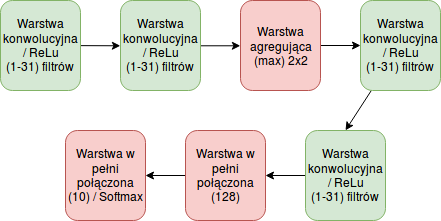
\includegraphics[width = 1.0\linewidth]{img/fenotyp}
	 \caption{Przedstawienie pojedynczego osobnika \\
              Źródło: praca własna}
	 \label{fig:fenotyp}
\end{figure}

Odgórnie osiągi zbioru sieci ograniczone są przez elementy ustalone, tj. czerwone elementy na rys. \ref{fig:fenotyp}, stałą liczbę warstw konwolucyjnych (4) oraz granice w jakich zmieniają się liczby filtrów w tychże (1-31).
Zadaniem algorytmu genetycznego będzie maksymalizacja jakości klasyfikacji obrazów tak opisanych sieci po jednej epoce uczenia.
Przy tak dobranych parametrach osobnika możliwe jest wystąpienie zjawiska nadmiernego dopasowania do zbioru uczącego przez otrzymane sieci, w związku z brakiem zastosowania środków zapobiegawczych (takich jak dropout).

Funkcja przystosowania dla pojedynczego osobnika, jak już wspomniano w \ref{sec:reduction}, została określona jako skuteczność sieci po jednej epoce uczenia.
Nic nie stałoby jednak na przeszkodzie, aby dodać inne kryteria do funkcji przystosowania, np. gdyby zależało nam na uzyskaniu sieci która zajmuje mało pamięci moglibyśmy odjąć od funkcji przystosowania odjąć odpowiednią karę proporcjonalną do sumy ilości wszystkich filtrów w warstwach.

\section{Operacje genetyczne algorytmu genetycznego}\label{sec:genetic_ops}
Spośród wymienionych w \ref{sec:ag} operacji genetycznych należało wybrać, jakie zaimplementować w programie realizującym algorytm genetyczny.
\subsection{Selekcja}
Wybranym w tej pracy sposobem selekcji jest sposób proporcjonalny, zwany również ruletkowym.
Każdy z osobników przypisany zostaje do obszaru ruletki, którego rozmiar jest proporcjonalny do wartości funkcji przystosowania tego osobnika.
Następnie $N$-krotnie kręci się ruletką, a pole, na które wypadnie, determinuje który z osobników przechodzi do puli potomków.
W ten sposób lepiej przystosowane osobniki mają większą szansę przejścia dalej i przekazania swoich genów.
W przypadku długotrwałego obliczania funkcji przystosowania dodatkową zaletą takiego podejścia jest większa szansa na pojawienie się takich samych osobników (które nie zostaną poddane krzyżowaniu ani mutacji) w kolejnej iteracji algorytmu.
Z punktu widzenia efektywniejszego przeszukiwania przestrzeni dostępnych rozwiązań nie jest to zaletą, jednakże pozwala oszczędzić obliczeń dla już obliczonych punktów.

Tutaj metoda proporcjonalna została zaimplementowana w następujący sposób:

Powtórz $N$-krotnie:
\begin{enumerate}
  \item sumowane są wartości funkcji przystosowania $S(\mathbf{x})=\sum_{i=1}^{N}f(x_i)$ dla każdego $x_i$ w populacji,
  \item losowana jest losowa liczba z przedziału $r = (0,S(\mathbf{x}))$,
  \item znajdowane jest najmniejsze $i$, dla którego w danej sekwencji osobników $\sum_{i=1}^{N}x_i > r $.
\end{enumerate}

\subsection{Krzyżowanie}
Przy implementacji algorytmu genetycznego wybrano krzyżowanie jednorodne.
Dla pary chromosomów rodzicielskich, które są w istocie dwoma ciągami binarnymi o jednakowej długości, losowana jest binarna maska o tej samej długości.
Następnie następuje zamiana miejscami bitów oznaczonymi jako 1 w wylosowanej masce, w wyniku czego powstają dwa nowe chromosomy - potomkowie.
Działanie to w sposób schematyczny przedstawiono na rys. \ref{fig:crossing}.
Rozważając poniższy przykład jako dwie warstwy konwolucyjne zakodowane na 4-bitach każdy, z rodziców $[12,3]$ oraz $[7,1]$ otrzymujemy z daną maską dwie nowe sieci z warstwami: $[5,3]$ oraz $[14,1]$.

\begin{figure}[h!tb]
	 \centering
	 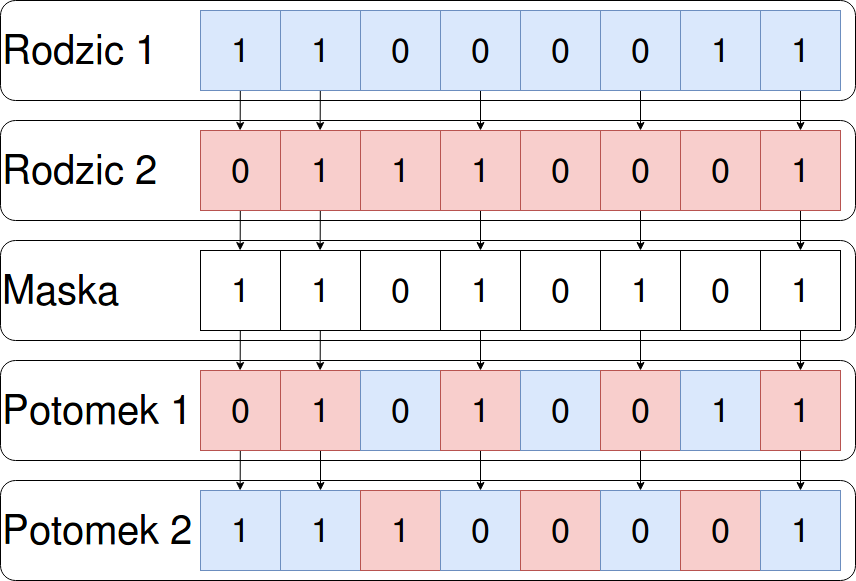
\includegraphics[width = 1.0\linewidth]{img/crossing}
	 \caption{Krzyżowanie jednorodne \\
              Źródło: praca własna}
	 \label{fig:crossing}
\end{figure}

\subsection{Mutacja}
Sposób mutacji wykorzystany w tej pracy tożsamy jest ze zmianą wartościowo-równomierną.
Dokonywana jest ona na fenotypie osobnika.
Jeżeli mutacja danego osobnika zachodzi, to:
\begin{itemize}
  \item losowo wybierana jest liczba ze zbioru $\lbrace 0, 1, 2, 3 \rbrace$, która determinuje, który parametr będzie zmieniany,
  \item następuje wylosowanie nowej wartości dla wybranego parametru z dopuszczalnego zbioru liczb całkowitych $\lbrace 1..31 \rbrace$, który zastępuje starą wartość.
\end{itemize}

\subsection{''Naprawianie'' osobników}\label{sec:individual_fix}
Istnieje pewne prawdopodobieństwo, że w wyniku krzyżowania otrzymamy osobnika, dla którego jeden lub więcej parametrów przyjmie wartość zero.
Rozwiązać ten problem można na dwa sposoby:
\begin{enumerate}
  \item na poziomie algorytmu genetycznego - zamieniając otrzymane 0 losową lub najbliższą (1) dopuszczalną wartością\label{bullet:genetic_fix},
  \item na poziomie konstruowania sieci neuronowej - jeżeli warstwa zawiera 0 filtrów to jest pomijana w sekwencyjnym budowaniu modelu sieci.
\end{enumerate}
W pracy zdecydowano się zastosować się podejście \ref{bullet:genetic_fix} z zastępowaniem 0 przez 1, ze względu na prostotę implementacji.

\subsection{Substytucja}
Zastosowana w algorytmie technika substytucji osobników rodzicielskich przez potomków jest strategią z reprodukcją częściową.
W celu zmniejszenia ilości obliczeń potomkowie nie są oceniani do momentu, kiedy staną się rodzicami w następnym pokoleniu.
Z tego powodu zastosowano połączenie strategii elitarnej (pozostawienie najlepszych osobników z poprzedniej iteracji) z zastępowaniem losowo wybranych osobników (losowo wybierane są nowe osobniki z puli potomków).
Pozwala to dodatkowo zaoszczędzić obliczeń dla przeniesionej z poprzedniej iteracji elity przy jednoczesnym zachowaniu różnorodności genetycznej pochodzącej od losowo wybranych potomków.
Dodatkowo, w stosunku do pełnej reprodukcji (z wymianą całej populacji), algorytm szybciej znajduje lepsze rozwiązania.

\section{Architektura eksperymentu}
W toku przygotowywania eksperymentów powstał system napisany w języku Python\cite{CS-R9526}.
Najważniejsze jego elementy zostały wyróżnione na rys. \ref{fig:system_overview}

\begin{figure}[h!tb]
	 \centering
	 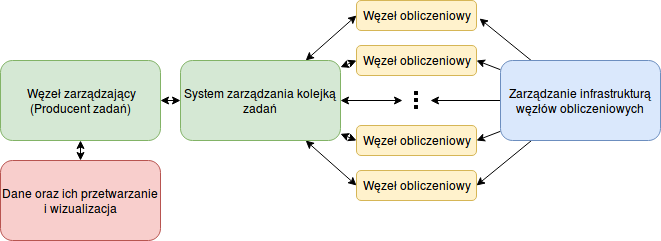
\includegraphics[width = 1.0\linewidth]{img/system_overview}
	 \caption{Całokształt systemu przeprowadzania eksperymentu \\
              Źródło: praca własna}
	 \label{fig:system_overview}
\end{figure}

Każdy z powyżej przedstawionych elementów zostanie omówiony dalej.
Poniżej, na rys. \ref{fig:folder_structure} przedstawiono strukturę katalogów projektu:

\begin{figure}[h!tb]
	 \centering
	 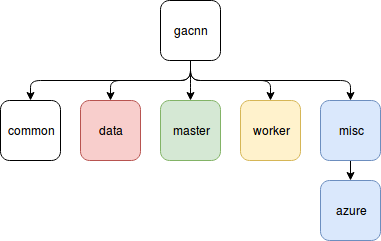
\includegraphics[width = 0.7\linewidth]{img/folder_structure}
	 \caption{Struktura katalogów projektu systemu eksperymentu\\
              Źródło: praca własna}
	 \label{fig:folder_structure}
\end{figure}

Całość projektu zorganizowano w katalogi tak, aby zgrupować pliki źródłowe powiązane z konkretnymi blokami funkcjonalnymi z rys. \ref{fig:system_overview}.
Bloki oznaczone na obydwu rysunkach tym samym kolorem są swoimi odpowiednikami.
W związku z tym:
\begin{itemize}
  \item katalog \textit{gacnn} jest korzeniem, również nazwą repozytorium kodu źródłowego,
        Jego nazwa jest abrewiacją angielskich odpowiedników nazw algorytm genetyczny i konwolucyjna sień neuronowa,
  \item katalog \textit{common} zawiera elementy potrzebne możliwie przez każdy z innych modułów,
  \item katalog \textit{data} przechowuje zebrane przez węzeł zarządzający dane oraz skrypty służące do ich przetwarzania i wizualizacji,
  \item katalog \textit{master} zawiera wszystkie programy, które mogą być węzłem zarządzającym, oraz system zarządzania kolejką zadań,
  \item katalog \textit{worker} zawiera oprogramowanie uruchamiane na każdym z węzłów obliczeniowych,
  \item katalog \textit{misc} zawiera pomocnicze skrypty służące do tworzenia i przygotowywania węzłów obliczeniowych,
  \item katalog \textit{azure} zawiera skrypty j.w. przeznaczone konkretnie do tworzenia instancji węzłów obliczeniowych na platformie Microsoft Azure.
\end{itemize}

\subsection{Elementy wspólne}
Wspólne elementy autorskiego kodu używane zarówno przez węzeł zarządzający, jak i przez węzły obliczeniowe, to definicje dwóch klas:
\begin{itemize}
  \item klasa \textit{Job} - opisuje zadane przekazywane przez węzeł zarządzający do systemu kolejkowego i dalej do węzła obliczeniowego.
        W istocie swej jest to struktura przechowująca 3 elementy:
        \begin{itemize}
          \item osobnika (reprezentowanego przez obiekt klasy \textit{Individual}), dla którego należy wyznaczyć funkcję przystosowania,
          \item liczbę epok uczenia sieci neuronowej,
          \item ziarno dla generatora pseudolosowego.
        \end{itemize}
  \item klasa \textit{Individual} - opisuje pojedynczego osobnika, tj. pojedynczą strukturę sieci neuronowej.
        Przechowuje ona 4 informacje:
        \begin{itemize}
          \item fenotyp osobnika - lista 4 liczb opisujących liczbę filtrów w odpowiednich warstwach sieci,
          \item przystosowanie osobnika - wartość funkcji przystosowania osobnika.
                Dla algorytmu optymalizującego strukturę konwolucyjnej sieci neuronowej jest to skuteczność klasyfikacji zbioru testowego przez nauczoną sieć,
          \item ostateczna uzyskana wartość funkcji kosztu (\textit{loss function}) po uczeniu - w celu informacyjnym,
          \item historię uczenia sieci - przechowuje wartości przystosowania i funkcji kosztu po każdej epoce uczenia sieci, przechowywane w celach informacyjno-diagnostycznych.
        \end{itemize}
\end{itemize}


\subsection{Węzeł zarządzający}

Węzłem zarządzającym nazywany będzie program, który korzysta z opisanego w \ref{sec:queue_system} systemu kolejkowego do rozdzielania swoich zadań i odbierania wyników.
Jego głównym zadaniem jest typowanie osobników, dla których ma zostać wyliczona funkcja przystosowania.
Dla potrzeb wspomnianych w \ref{sec:reduction} funkcji przystosowania dla uczenia 1- i 10- epokowego konieczne było stworzenie dwóch programów zarządzających:
\begin{enumerate}
  \item węzeł typujący osobniki do wyliczenia na podstawie działania algorytmu genetycznego dla uczenia 1-epokowego - plik \textit{genetic\_algorithm.py}\label{list:genetic},
  \item węzeł typujący najlepsze, środkowe i najgorsze osobniki z każdej iteracji algorytmu genetycznego dla uczenia 10-epokowego - plik \textit{full\_learning.py}\label{list:full}.
\end{enumerate}
Obydwa z wyżej wymienionych węzłów korzystają z pomocniczych funkcji do zapisywania odebranych od węzłów obliczeniowych danych - plik \textit{csv\_handling.py}.

Węzeł opisany powyżej w punkcie \ref{list:genetic} został napisany tak, by możliwie łatwo można było regulować parametry algorytmu.
Poniżej przedstawiono ich listę:
\begin{itemize}
  \item liczba osobników $N$,
  \item wymiarowość przestrzeni poszukiwań - liczba warstw konwolucyjnych $n$,
  \item zakres przestrzeni poszukiwań - liczba bitów przypadających na kodowanie jednej warstwy $m$,
  \item prawdopodobieństwo krzyżowania - $p_{c}$,
  \item prawdopodobieństwo mutacji - $p_{m}$,
  \item maksymalna liczba iteracji,
  \item maksymalna liczba iteracji bez poprawy,
  \item liczba najlepszych osobników przechodzących do kolejnego pokolenia - $ N_{k} = 30$,
  \item minimalna poprawa $\epsilon$,
  \item ziarno generatora pseudolosowego - domyślnie 1337.
\end{itemize}

Po ustawieniu wyżej wymienionych parametrów, program działa następująco:

\begin{enumerate}
  \item ustawia zadane ziarno generatora losowego. Przyczyny, dla których to robi, opisano w \ref{sec:replicativity}.
  \item jeśli nie istnieje, tworzy plik .csv do przechowywania danych, gdzie każdy wpis zawiera:
  \begin{itemize}
    \item numer iteracji,
    \item genotyp osobnika w formie zakodowanej,
    \item wartość funkcji przystosowania,
    \item wartość funkcji kosztu.
  \end{itemize}
  \item jeżeli istnieje plik .csv z danymi z niedokończonego działania programu, wczytuje je,
  \item jeżeli nie wczytano żadnych danych, następuje inicjalizacja populacji. Losowo generowanych jest $N$ osobników,
  \item dopóki nie osiągnięto kryterium stopu (maksymalna liczba iteracji bez poprawy wyniku lub maksymalna liczba iteracji osiągnięte):
  \begin{enumerate}
    \item przygotowuje listę zadań dla systemu kolejkowego - dla każdego osobnika tworzy jedno zadanie, które w jednym zdaniu brzmi: ''Ucz tego osobnika przez 1 epokę z takim ziarnem generatora pseudolosowego'',
    \item oblicza wartość funkcji przystosowania dla całej populacji korzystając z metody \textit{evaluate(jobs)} systemu kolejkowania zadań,
    \item sortuje osobniki według wartości funkcji przystosowania,
    \item zapisuje dane z tej iteracji do pliku csv,
    \item sprawdza najlepszy wynik i czy w tej iteracji nastąpiła poprawa - jeśli nie, zwiększa licznik iteracji bez poprawy,
    \item za starą populację podstawia nową uzyskaną w wyniku:
    \begin{enumerate}
      \item selekcji,
      \item krzyżowania,
      \item mutacji,
      \item ''naprawiania'' osobników,
      \item substytucji.
    \end{enumerate}
    Wszystkie z powyższych odbywają się jak opisano w \ref{sec:genetic_ops}.
  \end{enumerate}
\end{enumerate}

W wyniku działania powyższego skryptu otrzymujemy plik csv zawierający wszystkie osobniki z wszystkich iteracji działania algorytmu genetycznego.
Dane te są przetwarzane dalej w celu wizualizacji, jak również przez skrypt \textit{full\_learning.py}, który również jest węzłem zarządzającym, a działa następująco:
\begin{enumerate}
  \item wczytuje osobniki zapisane w pliku .csv przez algorytm genetycznych,
  \item z każdej iteracji wybiera najlepszego, środkowego i najgorszego osobnika,
  \item dla każdego wybranego osobnika tworzy zadanie, które w jednym zdaniu brzmi: ''Ucz tego osobnika przez 1 epokę z takim ziarnem generatora pseudolosowego'',
  \item oddelegowuje zadania do systemu kolejkowania zadań,
  \item zbiera wyniki i zapisuje je do innego pliku.
\end{enumerate}
Ten skrypt wyznacza inną funkcję przystosowania dla tych samych osobników - skuteczność po 10 epokach uczenia, w porównaniu do 1-epokowego uczenia.

\subsection{System kolejkowania zadań}\label{sec:queue_system}
W celu maksymalnego przyspieszenia obliczeń, dokonano zrównoleglenia obliczania funkcji przystosowania dla każdego osobnika.
Ze względu na ograniczoną liczbę jednostek obliczeniowych mogących jednocześnie przetwarzać żądania, zaprojektowano system kolejkowy.
Schemat tego systemu przedstawiono na rys. \ref{fig:queue_system}
\begin{figure}[h!tb]
	 \centering
	 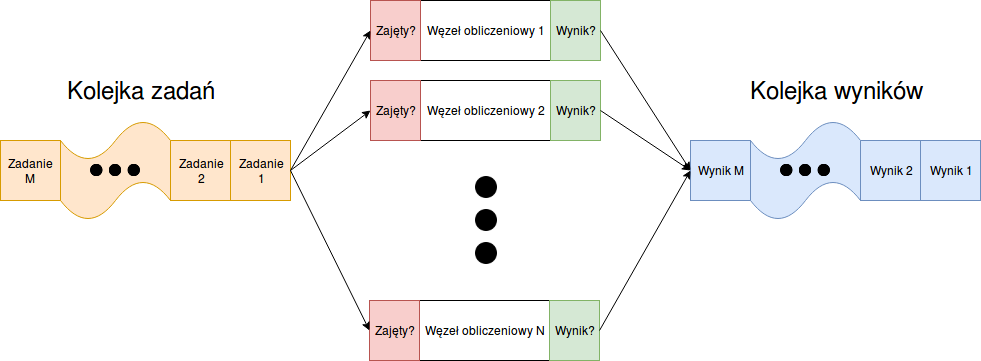
\includegraphics[width = 1.1\linewidth]{img/kolejkowanie}
	 \caption{System kolejkowania obliczeń \\
              Źródło: praca własna}
	 \label{fig:queue_system}
\end{figure}

Implementacja systemu kolejkowego zawarta jest w pliku \textit{queue\_handling.py}.
Zawiera on następujące elementy:

\begin{itemize}
  \item interfejs \textit{Worker} będącą reprezentacją pojedynczego węzła obliczeniowego,
  \item klasę \textit{RemoteWorker} dziedziczącą po klasie \textit{Worker}, służącą do delegowania zadań do zdalnej maszyny wirtualnej wykonującej obliczenia,
  \item klasę \textit{LevyWorker} dziedziczącą po klasie \textit{Worker}, lokalnie wyznaczającą wartość funkcji Levy'ego, używana przy testowaniu działania algorytmu genetycznego jak opisano w \ref{sec:levy_test},
  \item klasę \textit{WorkManager} będącą właściwą implementacją systemu kolejkowania.
\end{itemize}

Interfejs \textit{Worker} zawiera następujące metody:
\begin{itemize}
  \item \textit{is\_available()} - mówi, czy dany węzeł może przyjmować teraz zadania,
  \item \textit{assign\_job(job)} - przypisuje do danego węzła przekazane jako argument zadanie do obliczania,
  \item \textit{has\_result()} - odpytuje węzeł, czy posiada już wynik obliczeń,
  \item \textit{get\_result{}} - zwraca odebrany od węzła wynik obliczeń,
  \item \textit{free\_worker()} - zwalnia węzeł oznaczając go jako gotowy do rozpoczęcia dalszych obliczeń,
  \item \textit{get\_current\_job()} - zwraca aktualnie zlecone węzłowi zadanie.
\end{itemize}

Właściwą implementacją systemu kolejkowego jest klasa \textit{WorkManager}.
System kolejkowy przechowuje wewnętrznie listę dostępnych węzłów obliczeniowych.
Jedyną publiczną metodą tej klasy jest funkcja \textit{evaluate(jobs)}, która jako argument przyjmuje listę zadań do wykonania.
Dla przypadku obsługi węzłów zdalnych system kolejkowy:

\begin{enumerate}
  \item wyszukuje duplikaty wśród otrzymanych zadań i zawęża listę zadań do unikalnego zbioru\label{list:duplicates}
  \item dopóki liczba uzyskanych wyników jest mniejsza od liczby zleconych zadań:
    \begin{enumerate}
      \item sprawdza plik \textit{workers} z listą adresów IP potencjalnych węzłów,
      \item próbuje połączyć się z węzłami zgodnie z procedurą opisaną w \ref{sec:communication},
      \item dodaje każdy zgłaszający się węzeł do listy węzłów i oznacza go jako wolny,
      \item rozdziela zadania każdemu z węzłów, dla każdego węzła z listy:
        \begin{enumerate}
          \item sprawdza czy ten węzeł jest oznaczony jako wolny i czy są dostępne zadania,
                Jeśli nie, przechodzi do kolejnego węzła i powtarza obecny krok.
          \item pobiera zadanie z puli dostępnych zadań,
          \item próbuje przypisać pobrane zadanie do tego węzła (może się to nie udać np. z powodu utraty połączenia sieciowego),
          \item jeśli powyższy krok się nie powiódł, przywraca zadanie do puli zadań, a niedziałający węzeł jest usuwany z listy węzłów.
        \end{enumerate}
      \item odpytuje każdy zajęty węzeł o wyniki w następujący sposób:\label{enum:second_worker_check}
      \begin{enumerate}
        \item odpytuje węzeł czy wynik jest dostępny.
              Jeśli nie, przechodzi do kolejnego węzła i powtarza obecny krok.
        \item pobiera od węzła jego wynik i zadanie. Zapisuje je do słownika, gdzie zadanie jest kluczem, a wynik wartością,
        \item oznacza węzeł jako wolny,
        \item jeśli któryś z powyższych kroków się nie powiódł, przywraca zadanie węzła do puli i usuwa go z listy węzłów.
      \end{enumerate}
      \item w celu zmniejszenia obciążenia sieci przy komunikacji z węzłami, odczekuje sekundę przed kolejną iteracją.
    \end{enumerate}
  \item przywraca usunięte w punkcie \ref{list:duplicates} duplikaty, przepisując odpowiednie wyniki z policzonych zadań ze słownika zadanie-wynik.
\end{enumerate}

W przypadku testu dla lokalnie obliczane wartości funkcji Levy'ego opisanego w \ref{sec:levy_test} system ten, z pewnymi modyfikacjami, również może zostać wykorzystany.
Obliczenia wykonywane są lokalnie i dostępne są natychmiast po zleceniu zadania, w związku z czym:
\begin{itemize}
  \item lista węzłów zawiera tylko jeden węzeł \textit{LevyWorker} i nie jest w żaden sposób modyfikowana
  \item pominięte zostaje opóźnienie odciążające sieć
\end{itemize}

\subsection{Protokół komunikacji ze zdalnymi węzłami}\label{sec:communication}

Komunikacja ze zdalnymi węzłami odbywa się przez protokół TCP/IP z wykorzystaniem interfejsu \textit{socket} języka Python.

Schemat wymiany komunikatów przedstawiony został na rysunku \ref{fig:komunikacja}
\begin{figure}[h!tb]
	 \centering
	 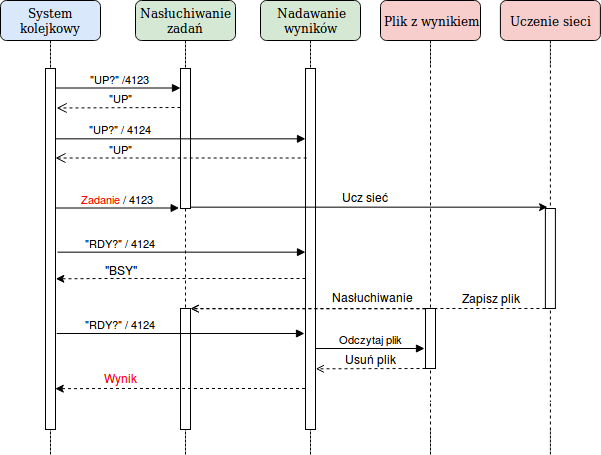
\includegraphics[width = 1.0\linewidth]{img/komunikacja}
	 \caption{Schemat wymiany komunikatów pomiędzy systemem kolejkowym a węzłami obliczeniowymi \\
              Źródło: praca własna}
	 \label{fig:komunikacja}
\end{figure}

Widoczne u góry bloki komunikują się ze sobą zgodnie ze schematem.
Pierwszy (niebieski) blok reprezentuje komunikujący się z węzłem obliczeniowym system kolejkowania zadań.
Pozostałe 4 bloki stanowią podsystem pojedynczego węzła obliczeniowego.
Na zielono zaznaczono obiekty komunikujące się przez sieć, natomiast na czerwono zaznaczono bloki niedostępne bezpośrednio z poziomu węzła zarządzającego.

Sama komunikacja przebiega w następujący sposób.
\begin{enumerate}
  \item system kolejkowy sprawdza, czy pod zadanym adresem IP rzeczywiście znajduje się węzeł obliczeniowy.
  Sprawdzenie to polega na przesłaniu tekstowo zapytania ''UP?'' na obydwa otwarte porty węzła obliczeniowego.
  Jeżeli w odpowiedzi z obydwu portu dostaje komunikat ''UP'', dodaje węzeł do swojej wewnętrznej listy węzłów i nie powtarza więcej tej komunikacji do momentu, kiedy znowu będzie potrzeba dodania tego węzła do listy,
  \item jeżeli poprzedni punkt przebiegł pomyślnie, węzeł jest gotowy do przyjęcia zadania.
  System kolejkowy przesyła spakowany przy pomocą modułu \textit{Pickle} obiekt klasy \textit{Job} na port 4123, który jest używany do akceptacji zadań,\label{list:job}
  \item następnie cyklicznie (co sekundę, jest to wspominane w \ref{sec:queue_system} opóźnienie przesyłane jest zapytanie na port 4124 czy jest już wynik poprzez komunikat ''RDY?''.
  Jeżeli wynik jeszcze nie jest dostępny, odsyłana jest odpowiedź ''BSY'' oznaczająca dalsze trwanie obliczeń.\label{list:result}
  W przeciwnym wypadku przesyłany jest spakowany przy pomocą modułu \textit{Pickle} obiekt klasy \textit{Individual} zawierający w sobie wyniki obliczeń,
  \item system kolejkowy następnie powtarza kroki \ref{list:job} i \ref{list:result} tak długo, jak posiada zadania do rozdzielenia, lub dopóki nie nastąpi nieoczekiwany błąd.
\end{enumerate}

\subsection{Węzeł obliczeniowy}\label{sec:worker_node}

Przez węzeł obliczeniowy rozumieć będziemy komputer lub maszynę wirtualną z dostępem do sieci komputerowej, w której znajduje się węzeł zarządzający.
Dodatkowym wymaganiem na taki węzeł jest możliwość uruchomienia na nim skryptów \textit{listener\_results.py} oraz \textit{listener\_jobs.py}, przy czym ten drugi powinien być cyklicznie uruchamiany w przypadku wystąpienia błędu.
Implikuje to obecność na danej maszynie interpretera języka Python w wersji 3 wraz z odpowiednimi bibliotekami, tj. \textit{TensorFlow}\cite{tensorflow2015-whitepaper}, \textit{Keras}\cite{chollet2015keras} oraz \textit{Numpy}\cite{ascher.dubois.hinsen.hugunin.oliphant-1999-np}.
Co więcej, urządzenie to musi mieć możliwość przyjmowania połączeń od systemu kolejkowego na portach TCP 4123 oraz TCP 4124.

Zadaniem węzła obliczeniowego jest przyjęcie zadania od systemu kolejkowego, wykonanie go i dostarczenie wyniku, również na żądanie systemu kolejkowego, przy spełnianiu wyspecyfikowanego w \ref{sec:communication} protokołu komunikacyjnego.
W związku z tym kod uruchamiany na węźle został rozdzielony na 3 pliki źródłowe, każdy odpowiedzialny za jedno z tych zadań.

Pierwszym z nich jest \textit{listener\_jobs.py}.
Działa on według następującego schematu:
\begin{enumerate}
  \item ustawia socket nasłuchujący połączeń na porcie TCP/4123
  \item w nieskończonej pętli:
  \begin{enumerate}
    \item akceptuje przychodzące połączenie i odbiera dane,
    \item jeżeli w przychodzących danych występuje komunikat ''UP?'' odsyła komunikat ''UP'', zamyka połączenie i pomija resztę kroków w tym przebiegu pętli,
    \item zamyka połączenie od systemu kolejkowego,
    \item rozpakowuje przychodzące dane i sprawdza czy otrzymano obiekt klasy \textit{Job}, w przeciwnym wypadku generuje wyjątek i zakańcza działanie programu,
    \item przekazuje sterowanie do funkcji \textit{eval\_network(...)} z parametrami odczytanymi z otrzymanego obiektu.
  \end{enumerate}
\end{enumerate}

Na czas uczenia sieci proces nie nasłuchuje połączeń - przyjęto założenie projektowe, że to system zarządzający kolejką przechowuje informację, że ten węzeł właśnie pracuje i zostanie zwolniony po odebraniu wyników.

Kolejny plik, tj. \textit{eval\_cnn.py}, zawiera jedną metodę, która oblicza funkcję przystosowania osobnika, poprzez skonstruowanie modelu sieci, uczenie go zbiorem uczącym oraz walidację na zbiorze testowym obrazków ze zbioru CIFAR-10.
Bardziej szczegółowo:
\begin{enumerate}
  \item ustawia zadane ziarno generatora losowego. Przyczyny, dla których to robi, opisano w \ref{sec:replicativity},
  \item ładuje do pamięci zbiór danych CIFAR-10. Jeżeli skrypt jest uruchamiany pierwszy raz, pobiera ów zbiór z internetu,
  \item buduje model sieci neuronowej taki jak przedstawiono na rys. \ref{fig:fenotyp}.
        Budowanie modelu jest uniwersalne dla różnych długości fenotypu, tj. różnej zadanej ilości warstw konwolucyjnych.
        Warstwa agregująca zostanie wstawiona w połowie , czyli dla 4 warstw za 2. warstwą.
  \item uczy uzyskany model korzystając z optymalizatora \textit{RMSProp} przez zadaną liczbę epok. Otrzymaną historię uczenia przechowuje w odpowiednim polu obiektu klasy \textit{Individual},\label{list:training}
  \item sprawdza skuteczność uzyskanej nauczonej sieci na zbiorze testowym, j.w. zapisując uzyskaną skuteczność i wartość funkcji kosztu w odpowiednich polach,\label{list:check}
  \item pakuje uzupełniony przez powyższe operacje obiekt klasy \textit{Individual} przy pomocy modułu \textit{pickle} i zapisuje wynik w pliku ''result''.
\end{enumerate}

Przy przeprowadzaniu eksperymentów zaobserwowano niedeterministyczne występowanie wyjątku \textit{MemoryError} oznaczającego zużycie całej dostępnej pamięci i brak miejsca na alokowanie nowej, powodujący zakończenie działania programu.
Prawdopodobną przyczyną jest błąd programistyczny w jednej z użytych bibliotek.
Zastosowanym sposobem obejścia tego problemu jest ponowne uruchomienie skryptu przez inny skrypt.

Trzeci plik \textit{listener\_results.py} odpowiedzialny jest za przesyłanie wyników na żądanie systemu kolejkowego lub informowanie, że nie są one jeszcze dostępne.
Program ten realizuje następujące kroki:
\begin{enumerate}
  \item ustawia socket nasłuchujący połączeń na porcie TCP/4124,
  \item w nieskończonej pętli:
  \begin{enumerate}
    \item akceptuje przychodzące połączenie i odbiera dane,
    \item jeżeli w przychodzących danych występuje komunikat ''UP?'' odsyła komunikat ''UP''. Jeżeli warunek nie jest spełniony, sprawdzany jest warunek poniżej,
    \item jeżeli w przychodzących danych występuje komunikat ''RDY?'' sprawdza czy jest dostępny plik z wynikami. Jeżeli nie, przesyła w odpowiedzi komunikat ''BSY''. Jeżeli jest, wysyła odczytany plik z wynikami,
    \item zamyka połączenie z systemem kolejkowym.
  \end{enumerate}
\end{enumerate}

Do poprawnego działania węzła obliczeniowego konieczne jest współbieżne uruchomienie skryptów \textit{listener\_results.py} oraz \textit{listener\_jobs.py}.
Co więcej, w związku ze wspomnianymi niedeterministycznymi błędami przy obliczaniu wartości funkcji przystosowania, program zbierający zadania powinien być restartowany po każdym krytycznym błędzie.
W związku z wykorzystaniem maszyn wirtualnych opartych o system Linux, w celu spełnienia dwóch powyższych warunków napisany został skrypt w języku Bash o nazwie \textit{starter.sh}.
Aby węzeł obliczeniowy zaczął działać, należy uruchomić w tle ten skrypt.
Jego działanie opisać można następująco:
\begin{enumerate}
  \item usuń plik z wynikami - zakładamy, że startujemy od nowa i nie powinno być wyników - realizowane przez komendę \textit{rm result},
  \item wyłącz działające procesy nasłuchujące zadań i wyników - realizowane przez komendę \textit{pkill python},
  \item uruchom w tle i uniezależnij od procesu rodzica skrypt \textit{listener\_results.py},
  \item w nieskończonej pętli:
  \begin{enumerate}
    \item uruchom skrypt \textit{listener\_jobs.py} i czekaj na jego wykonanie,
    \item poczekaj 10 sekund - oczekiwanie przed kolejnym uruchomieniem programu w przypadku, gdyby zajęty port TCP/4123 nie został jeszcze zwolniony.
  \end{enumerate}
\end{enumerate}

Tak złożony system spełnia warunki postawione na węzeł obliczeniowy.
Schematyczną jego reprezentację przedstawiono na rys. \ref{fig:worker_node}.
Każdy element wewnątrz prostokąta reprezentuje jeden z plików w folderze \textit{worker}.
Linia przerywana pomiędzy blokami \textit{listener\_results.py} a \textit{starter.sh} oznacza jedno uruchomienie.
Z kolei cykl pomiędzy \textit{listener\_jobs.py} a \textit{starter.sh} symbolizuje ponowne uruchamianie skryptu.
Na niebiesko zaznaczano współbieżnie dziejące skrypty komunikujące się z siecią.
Na czerwono zaznaczono elementy wykorzystywane wewnętrznie przez węzeł obliczeniowy.
Na zielono zaznaczono element rozpoczynający działanie systemu.
\begin{figure}[h!tb]
	 \centering
	 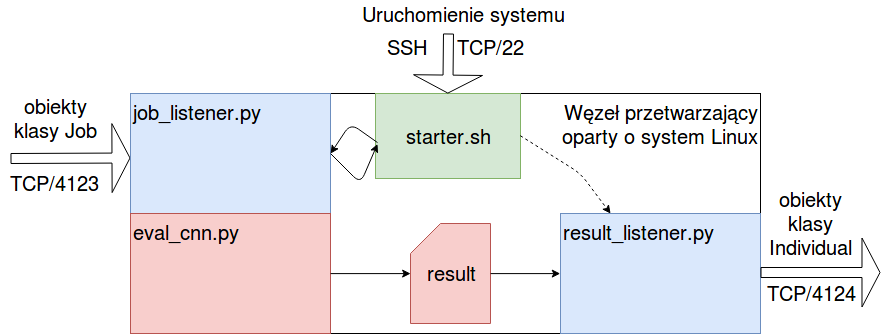
\includegraphics[width = 1.0\linewidth]{img/worker_node}
	 \caption{Schemat systemu obsługi zadań \\
              Źródło: praca własna}
	 \label{fig:worker_node}
\end{figure}

\subsection{Zarządzanie infrastrukturą węzłów obliczeniowych}\label{sec:azure}
Opisanym w \ref{sec:worker_node} węzłem obliczeniowym może być, jak wspomniano tamże, dowolna maszyna z systemem operacyjnym wspierającym uruchamianie równolegle procesów interpretera języka Python.
Dobrym rozwiązaniem okazują się być maszyny wirtualne z systemem Linux w chmurze.
Poniżej przedstawiono listę kilku dostawców takiego rozwiązania, których rozważano przy do stworzenia infrastruktury węzłów obliczeniowych:

\begin{itemize}
  \item Amazon Web Services,
  \item Microsoft Azure,
  \item Google Cloud Platform,
  \item DigtalOcean,
  \item Oktawave,
  \item OVH.
\end{itemize}

Na dzień dzisiejszy firma \textit{Microsoft} oferuje 100\$ kredytu do wykorzystania dla studentów w celach badawczych, dlatego rozwiązanie to zostało wykorzystane do utworzenia 20 instancji maszyn wirtualnych, które wykorzystano jako węzły obliczeniowe.
Subskrypcja dla studentów ma jednak pewne ograniczenia.
W trakcie prototypowego tworzenia infrastruktury napotkano ograniczenie możliwości działających vCPU w jednym regionie do 4.
Tym samym nie można było korzystać z maszyn wirtualnych wyposażonych w więcej vCPU, między innymi z przedstawionych w tabeli \ref{tab:gpu_optimized_vms}

\begin{table}[h!tb]
\centering
\small
\caption{Maszyny wirtualne zoptymalizowane pod kątem głębokiego uczenia. Źródło: \cite{gpuvms2018}}\label{tab:gpu_optimized_vms}
\begin{tabularx}{\linewidth}[c]{|l|X|X|X|X|X|X|X|X|X|} \hline
  Rozmiar & vCPU & Pamięć [GiB] & Pojemność tymczasowa (SSD) [GiB] & GPU & Maksymalnie dysków z danymi & Maksymalnie kart sieciowych \\ \hline
  Standard\_ND6s & 6 & 112 & 736 & 1 & 12 & 4 \\ \hline
  Standard\_ND12s &	12 & 224 & 1474 & 2 & 24 & 8 \\ \hline
  Standard\_ND24s & 24 & 448 & 2948 & 4 & 32 & 8 \\ \hline
 	\noalign{\smallskip}
\end{tabularx}
\vspace{-8pt}
\end{table}

Blok zarządzania infrastrukturą węzłów obliczeniowych widoczny na rys. \ref{fig:system_overview} po prawej stronie może reprezentować człowieka - operatora, który ręcznie utworzy wszystkie instancje korzystając z dostępnego na stronie \url{http://portal.azure.com} interfejsu WWW.
Na rys. \ref{fig:azure} przedstawiono interfejs webowy \textit{Microsoft Azure}.

\begin{figure}[h!tb]
	 \centering
	 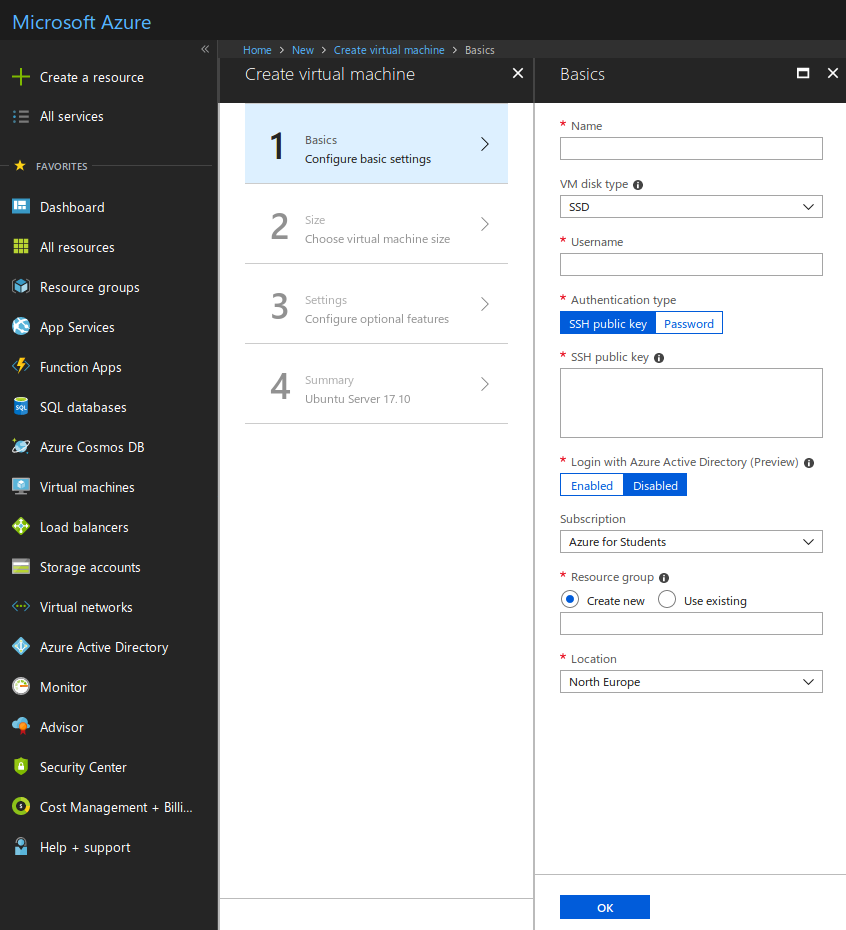
\includegraphics[width = 1.0\linewidth]{img/azure}
	 \caption{Interfejs Microsoft Azure - tworzenie maszyny wirtualnej \\
              Źródło: praca własna}
	 \label{fig:azure}
\end{figure}

Jak widać, oprócz początkowego wybrania obrazu (tutaj wybrano Ubuntu 17.10) należy przejść przez 4 etapy, gdzie musi podjąć następujące kroki:
\begin{enumerate}
  \item wprowadzić nazwę maszyny wirtualnej, np. \textit{Worker1},
  \item wprowadzić dane do logowania przez ssh: nazwę użytkownika i klucz publiczny,
  \item wybrać lub stworzyć grupę zasobów (nazwano grupę \textit{gacnn}),
  \item lokalizację - przy czym należy pamiętać o limicie 4 vCPU na lokalizację,
  \item wybrać rozmiar maszyny wirtualnej - tutaj wybrano rozmiar nazwany \textbf{DS1\_v2} o następujących parametrach:
  \begin{itemize}
    \item liczba vCPU: 1,
    \item pamięć RAM: 3.5 GB,
    \item rozmiar lokalnego SSD: 7 GB,
    \item cena: 41.41€ za miesiąc (0.0557€ za godzinę).
  \end{itemize}
  \item raz w każdym regionie stworzyć zestaw reguł zapory ogniowej (\textit{Network Security Group}) i dodać do niego regułę akceptującą połączenia na portach TCP: 4123-4124,
  \item przypisać utworzony powyżej zestaw reguł do tworzonej maszyny wirtualnej,
  \item wyłączyć niepotrzebną opcję diagnostyki uruchamiania (\textit{Boot Diagnostics}),
  \item zatwierdzić utworzenie maszyny wirtualnej.
\end{enumerate}
Rozwiązanie takie jest jednak czasochłonne i nieefektywne, przejście przez wszystkie etapy przy dużym poziomie koncentracji operatora zajmuje ok. ~3 minuty, co oznacza, że utworzenie 20 maszyn wirtualnych zajęłoby około godziny.

Rozwiązaniem tego problemu jest wykorzystanie narzędzia \textit{Azure CLI}, czyli interfejs linii komend dla Azure.
Pozwala on na zarządzanie maszynami wirtualnymi przy pomocy komend wydawanych z linii poleceń lub z poziomu skryptów napisanych w języku \textit{Bash} lub \textit{PowerShell}.
Zostały napisane dwa skrypty w języku bash.
Pierwszy to \textit{spawner.sh}, który tworzy 20 maszyn wirtualnych w 5 regionach po 4 maszyny za pomocą następującej komendy wywoływanej w pętli:\\

\begin{lstlisting}
az vm create --location $region --name $name
             --resource-group gacnn --size Standard_DS1_v2
             --image Canonical:UbuntuServer:17.10:latest
             --admin-username admin
             --ssh-key-value id_rsa.pub
             --no-wait
\end{lstlisting}

Zmienna \textit{region} przyjmuje jedną z wartości: \textit{northeurope, westeurope, francecentral, eastus, eastus2}.

Zmienna \textit{name} tworzona jest w następujący sposób:

\begin{lstlisting}
name=$region"worker"$i
\end{lstlisting}

Dzięki tej tworzone jest 20 maszyn o rozmiarze \textbf{DS1\_v2} o unikalnych nazwach.
Każda przypisywana jest do grupy zasobów \textit{gacnn}.
Wytwarzane są na podstawie najnowszego dostępnego obrazu \textit{Ubuntu Server 17}.
Logowanie do takiej maszyny możliwe jest z loginem admin i wyłącznie przy pomocy klucza publicznego z pliku \textit{id\_rsa.pub}.

Po utworzeniu maszyn należy im również otworzyć odpowiednie porty, odbywa się to przy pomocy komendy wywoływanej w pętli:
\begin{lstlisting}
az vm open-port --port 4123-4124 --resource-group gacnn --name $name
\end{lstlisting}

Z tak przygotowanymi maszynami można się połączyć przy pomocy programu, który pozwala obsługiwać wiele terminali naraz, np. \textit{Cluster SSH}.
Adresy IP maszyn odczytać można korzystając już z interfejsu WWW Azure, wyświetlając wszystkie dostępne maszyny wirtualne i ich publiczne adresy IP.
Poniższe kroki można w ten sposób wykonywać na 20 maszynach jednocześnie.

Dalsze przygotowanie środowiska dla węzła obliczeniowego polega na:
\begin{enumerate}
  \item pobraniu programu \textit{python3-pip},
  \item instalacja za jego pomocą bibliotek \textit{numpy, tensorflow, keras},
  \item sklonowanie repozytorium umieszczonego pod adresem \url{https://github.com/opiechow/gacnn},
  \item przejście do katalogu gacnn/worker,
  \item uruchomienie skryptu starer.sh.
\end{enumerate}

Po tych operacjach węzły obliczeniowe działają i czekają na zadania od systemu kolejkowego.
Można zmodyfikować plik \textit{starter.sh}, aby przekierować wyjście ze skryptu \textit{listener\_jobs.py} na standardowe wyjście, co pozwoli obserwować proces uczenia w terminalu.
Przykładowy widok dla sześciu węzłów obliczeniowych przedstawiono na rys. \ref{fig:wip}

\begin{figure}[h!tb]
	 \centering
	 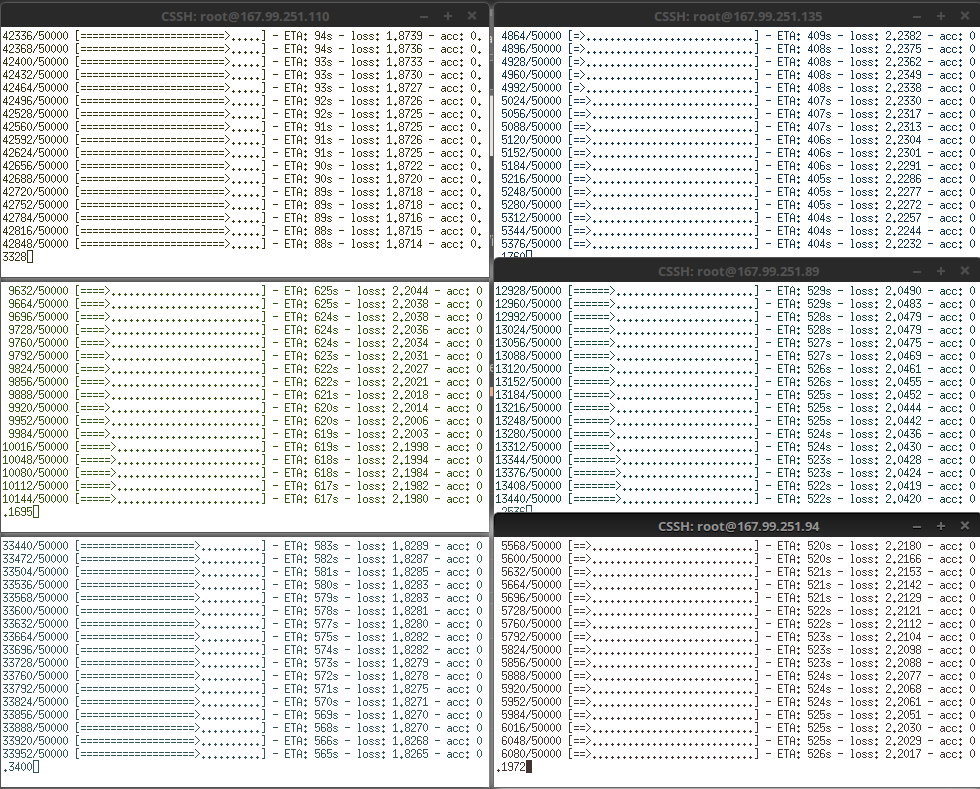
\includegraphics[width = 1.0\linewidth]{img/wip}
	 \caption{6 węzłów obliczeniowych w trakcie pracy \\
              Źródło: praca własna}
	 \label{fig:wip}
\end{figure}

\section{Replikacja badań}\label{sec:replicativity}
Zarówno w przypadku działania algorytmu genetycznego, jak i w przypadku uczenia sieci neuronowych, występuje wiele operacji, które z założenia powinny być niedeterministyczne.
Poniżej przedstawiono listę tych operacji dla algorytmu genetycznego:
\begin{itemize}
  \item losowe generowanie początkowej populacji algorytmu genetycznego,
  \item selekcja ruletkowa,
  \item losowe dobieranie osobników w pary rodzicielskie,
  \item zachodzenie krzyżowania z pewnym prawdopodobieństwem,
  \item losowanie maski w krzyżowaniu równomiernym,
  \item zachodzenie mutacji z pewnym prawdopodobieństwem,
  \item losowanie parametru do zmutowaniu,
  \item losowanie nowej wartości mutowanego parametru,
  \item losowanie części populacji przechodzącej do kolejnej iteracji.
\end{itemize}

W przypadku uczenia sieci neuronowych losowo inicjalizowane są początkowe wagi w sieci.

Aby zapewnić możliwość replikacji badań, w toku pisania systemu dbano o zachowanie kontroli nad stanem początkowym generatora liczb pseudolosowych.
W tym celu zarówno przed uruchomieniem algorytmu genetycznego jak i uczeniem sieci ustawiane jest ziarno generatora losowego.
W przypadku węzła zarządzającego ziarno jest jednym z parametrów ustawianym przed uruchomieniem algorytmu.
W przypadku węzłów obliczeniowych ziarno dla generatora odbierane jest razem z zadaniem do policzenia.

W przypadku algorytmu genetycznego używany jest generator z wbudowanego w język \textit{Python} modułu \textit{random}, ustawienie ziarna nie jest skomplikowane - wystarczy jedna linia kodu.
W przypadku uczenia sieci neuronowych wszystkie operacje losowe ukryte są w działaniu funkcji biblioteki \textit{Keras}.
Procedura ustawiania ziarna dla wszystkich generatorów dostępna jest w dokumentacji biblioteki. \cite{chollet2015keras}

Poważną wadą dbania o możliwość replikacji jest wymuszenie na \textit{TensorFlow} działania wyłącznie na jednym wątku, gdyż uniemożliwia to korzystanie z korzyści oferowanych przez uczenie sieci przy pomocy GPU i technologii CUDA.
Aby umożliwić działanie systemu w tymi technologiami, kryterium stopu uzależniono od wariancji wyników uzyskanych dla takiej samej sieci korzystając z różnych wartości ziarna generatora liczb losowych.

W przypadku przedstawionych poniżej eksperymentów nie korzystano z uczenia GPU, a z 20 maszyn wirtualnych z jednym vCPU każda.
Ziarno ustawiane było wg. opisanej powyżej procedury, zatem wszystkie badania powinny być możliwe do odtworzenia w sposób dokładny.

\chapter{Badania i testy}\label{chap:tests}
\section{Wariancja wyników dla jednej sieci}\label{sec:std_dev}
Ważnym parametrem algorytmu genetycznego jest jego kryterium stopu.
W przypadku eksperymentów opisanych w \ref{sec:levy_test} i \ref{sec:actual_experiment} przyjęto dwa:
\begin{enumerate}
  \item maksymalna liczba iteracji - z przyczyn długiego czasu potrzebenego na obliczenia w przypadku eksperymentu \ref{sec:actual_experiment}, liczbę tę ustalono na 100.
  \item maksymalna liczba iteracji bez poprawy - jeżeli od dłuższego czasu nie obserwujemy poprawy rozwiązania, możemy przyjąć założenie, że znaleźliśmy globalne minimum\label{improvement}
\end{enumerate}
Z punktem \ref{improvement} wiąże się parametr $\epsilon$, który ma sens progu różnicy między nową najlepszą wartością a poprzednią, po przekroczeniu którego możemy mówić o poprawie.

Program eksperymentu został tak zaimplementowany, by reprodukowalność eksperymentu była możliwie najwyższa, tj. by niwelować wpływ generatora pseudolosowego na uzyskane wyniki.
W procesie uczenia sieci neuronowych losowo inicjalizowane są wagi połączeń między neuronami.
Oznacza to, że w przypadku, gdy nie mamym kontroli nad stanem generatora losowego, ta sama w sensie struktury sieć może uzyskać inny wynik po jednej epoce uczenia w zależności od początkowych wag.

W celu minimalizacji wpływu losowego początkowego doboru wag na poprawę wyników sieci, przeprowadzono 100-krotnie uczenie sieci o 4 warstwach, po jednym filtrze w każdej, z różnymi początkowymi wagami.

Następnie wyznaczono wartość średnią (wzór \ref{eqn:mean}) wariancję (wzór \ref{eqn:variance}) zebranych pomiarów.

\begin{equation}\label{eqn:mean}
  \bar{x} = \frac{1}{N} \sum_{i=1}^{N} x_i
\end{equation}

\begin{equation}\label{eqn:variance}
  \sigma^2 = \frac{1}{N} \sum_{i=1}^{N}(x_i - \bar{x})^2
\end{equation}

Dla 100 prób wariancja wyniosła $\sigma^2 =3.708 \times 10^{-6}$, a odchylenie standardowe (pierwiastek kwadratowy z wariancji) $\sigma =1.9255 \times 10^{-3}$.
W związku z tym przyjęto wartość parametru $\epsilon = 4\sigma = 7.702 \times 10^{-3}$, aby wpływ różnej inicjalizacji wag nie był interpretowany przez algorytm genetyczny jako poprawa.

\section{Test działania algorytmu genetycznego}\label{sec:levy_test}
W celu zbadania poprawności działania oraz dostrojenia parametrów algorytmu genetycznego przeprowadzono test szukania minimum funkcji Levego.
Funkcja Levego (\textit{Levy Function}) dana jest wzorem \ref{eqn:levyfunction}:

\begin{equation}\label{eqn:levyfunction}
  f(\mathbf{x}) = sin^2(\pi w_1) + \sum_{i=1}^{d-1} (w_i - 1)^2 [ 1 + 10sin^2(\pi w_i + 1)] + (w_d - 1)^2 [1 + sin^2(2 \pi w_d)]
\end{equation}
gdzie $w_i$ obliczane jest ze wzoru \ref{eqn:wparam}, natomiast d oznacza liczbę wymiarów.
\begin{equation}\label{eqn:wparam}
  w_i = 1 + \frac{x_i - 1}{4}
\end{equation}

Minimum globalne tej funkcji znajduje się w punkcie $ \mathbf{x^*} = (1, ..., 1) $ a jego wartość wynosi zero, tj. $ f(\mathbf{x^*}) = 0 $. \cite{simulationlib}
Wykres tej funkcji dla przypadku 2-wymiarowego przedstawiono na rys. \ref{fig:levyfunction}

\begin{figure}[h!tb]
	 \centering
	 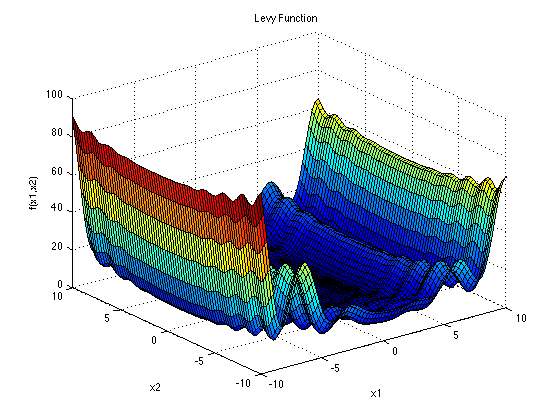
\includegraphics[width = 1.0\linewidth]{img/levy}
	 \caption{Wykres funkcji Levego \\
              Źródło: \cite{simulationlib}}
	 \label{fig:levyfunction}
\end{figure}

Przestrzeń poszukiwań (genotyp osobnika) przyjęto identyczną jak dla problemu optymalizacji struktury konwonlucyjnych sieci neuronowych, tj. $x_i \in \lbrace 1, 2, ... 30, 31 \rbrace$ dla $i = 1..4$.

W celu uniknięcia przypadku, w którym optymalny osobnik powstaje w wyniku mechanizmu naprawiania osbników (opisanego w \ref{sec:individual_fix}) dokonano arbitralnie dobranego przesunięcia wektora $\mathbf{x}$ o wektor $\begin{bmatrix}3 \\ 7 \\ 13 \\ 20\end{bmatrix}$, tak, że optymalne rozwiązanie znalazło się w punkcie $\mathbf{x^*} = \begin{bmatrix}4 \\ 8 \\ 14 \\ 21\end{bmatrix}$.

Jako, że algorytm maksymalizuje funkcję przystosowania osobników, w celu minimalizacji wartości funkcji Levego (funkcji kosztu) została ona zdefiniowana zgodnie ze wzorem \ref{eqn:levy_fitness}. \cite{bialaszewski2012}
\begin{equation}\label{eqn:levy_fitness}
  g(\mathbf{x}) = C_{max} - f(\mathbf{x})
\end{equation}
gdzie $C_{max} = 1000$ w celu spełnienia warunku $g(\textbf{x}) > 0$ dla każdego $\textbf{x}$ w przestrzeni poszukiwań.

Metodą prób i błędów dobrano takie nastawy parametrów algorytmu genetycznego, by znajdował on minimum tej funkcji, tj.
\begin{itemize}
  \item Liczba osobników $N = 100$
  \item prawdopodobieństwo krzyżowania - $p_{c} = 0.9$
  \item prawdopodobieństwo mutacji - $p_{m} = 0.3$
  \item maksymalna liczba iteracji - 100
  \item maksymalna liczba iteracji bez poprawy - 50
  \item liczba najlepszych osobników przechodzących do kolejnego pokolenia - $ N_{k} = 30$
  \item minimalna poprawa $\epsilon = 0.007702$
\end{itemize}

Ostatni parametr dobrany został w sposób opisany w \ref{sec:std_dev}
Operacje genetyczne przeprowadzane są tak jak opisano w \ref{sec:genetic_ops}.
Fenotyp pojedycznego osobnika jest 4-elementową listą liczb całkowitych: $[ x_1, x_2, x_3, x_4]$, natomiast genotyp jest binarną reprezntacją fenotypu na liczbach o długości $m=5$ bitów.
Badanie zostało przeprowadzone dla ziarna generatora ustawionego na wartość 1337.

Na rys. \ref{fig:levy_maxes} i rys. \ref{fig:levy_means} przestawiono odpowiednio maksymalne i średnie (dla całej populacji) wartości funkcji przystosowania w kolejnych iteracjach algorytmu.
Wszystkie kolejne wykresy zostały wykonane przy pomocy biblioteki \textit{Matplotlib}. \cite{Hunter:2007}

\begin{figure}[h!tb]
	 \centering
	 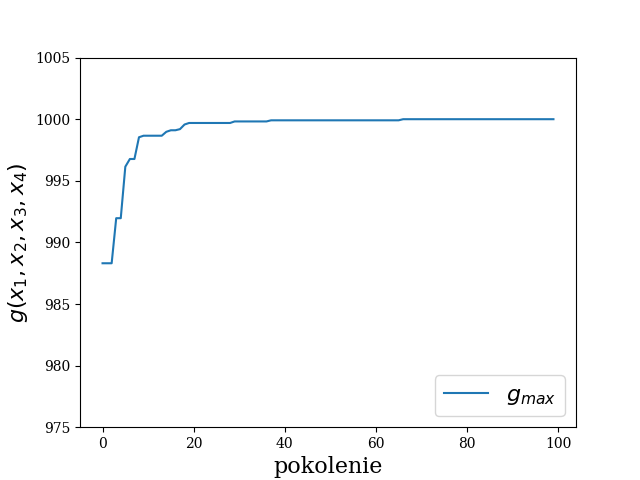
\includegraphics[width = 0.85\linewidth]{img/levy_maxes}
	 \caption{Maksymalne wartości funkcji przystosowania w każdej iteracji dla funkcji Levego \\
              Źródło: praca własna}
	 \label{fig:levy_maxes}
\end{figure}

\begin{figure}[h!tb]
	 \centering
	 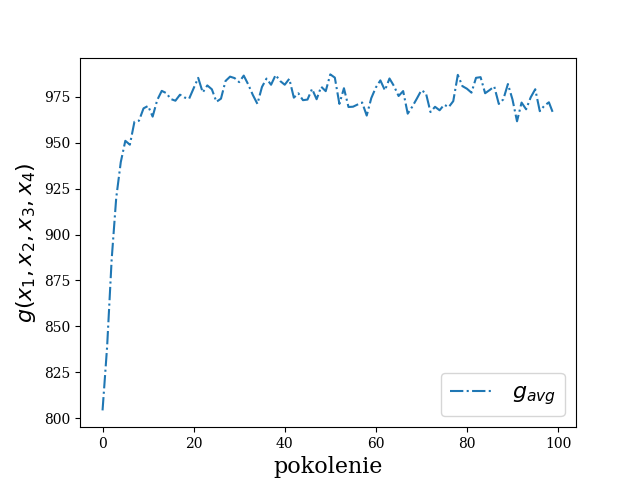
\includegraphics[width = 0.85\linewidth]{img/levy_means}
	 \caption{Średnie wartości funkcji przystosowania w każdej iteracji dla funkcji Levego \\
              Źródło: praca własna}
	 \label{fig:levy_means}
\end{figure}

Zaobserwowane przebiegi wyglądaja jak poprawne przebiegi dla algorytmu genetycznego.
Minimum w punkcie $\mathbf{x^*} = \begin{bmatrix}4 \\ 8 \\ 14 \\ 21\end{bmatrix}$ zostało znalezione w 67. pokoleniu, a kryterium zatrzymania algorytmu, które zadziałało, to maksymalna liczba iteracji równa 100.

Test ten udowodnił, że algorytm genetyczny został zaimplementowany poprawnie i w związku z tym można go w takiej formie wykorzystać do poszukiwania optymalnej struktury konwolucyjnych sieci neuronowych.

\section{Test działania dla lokalnego węzła obliczeniowego}

Schemat działania testu przedstawiono na rys. \ref{fig:localhost_test}

\begin{figure}[h!tb]
	 \centering
	 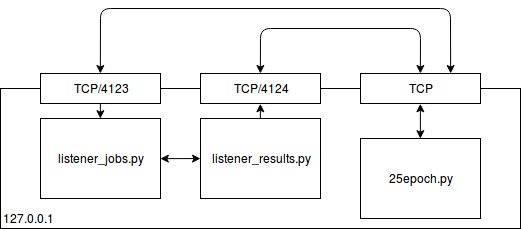
\includegraphics[width = 1.0\linewidth]{img/localhost_test}
	 \caption{Test działania całego systemu w ramach maszyny lokalnej\\
              Źródło: praca własna}
	 \label{fig:localhost_test}
\end{figure}

Kolejność wykonywania działań w teście była następująca:

\begin{enumerate}
  \item Modyfikacja pliku \textit{workers} by zawierał wyłącznie adres 127.0.0.1, czyli adres maszyny lokalnej
  \item Uruchomienie skryptu \textit{listener\_jobs.py} do nasłuchiwania zadań
  \item Uruchomienie skryptu \textit{listener\_jobs.py} do nasłuchiwania zapytań o wyniki
  \item Uruchomienie skryptu \textit{25epoch.py}, który zleca zadanie uczenia jednej sieci przez 25 epok
\end{enumerate}

Test ten pozwolił na zweryfikowanie:
\begin{enumerate}
  \item Czy rzeczywiście program węzła zdalnego działa niezależnie od systemu operacyjnego - na maszynie lokalnej działał system Linux Mint 18.3 Cinnamon 64 bit
  \item Czy zdefiniowano wystarczająco duży bufor dla przesyłu informacji pomiędzy węzłami
  \item Czy system kolejkowy działa jak powinien
\end{enumerate}

W wyniku działania testu zauważono, że bufor o rozmiarze 1 kiB (1024 bajtów) nie był wystarczająco duży, gdyż przesyłany plik z historią uczenia dla 25 epok miał rozmiar 1,5kB, co powodowało ucięcie transmisji i błąd w dekodowaniu spakowanego obiektu.
Dla zachowania pewnego zapasu bezpieczeństwa zwiększono rozmiar tego bufora do 8192 bajtów.

Ponadto test sprawdził działanie zarówno systemu kolejkowego dla brzegowego przypadku jednego zadania i jednego węxła, jak i oprogramowania węzła obliczeniowego.
W wyniku jego przeprowadzenia otrzymano poprawnie nauczoną sieć neuronową, więcej na ten temat powiedziano w \ref{sec:2525_epoch_training}.

\section{Poszukiwanie optymalnej struktury konwolucyjnej sieci neuronowej za pomocą algorytmu genetycznego dla uczenia 1-epokowego}\label{sec:actual_experiment}
Celem tego badania jest sprawdzenie, czy algorytm genetyczny jest w stanie znaleźć optymalną w sensie skutecznośći po jednej epoce uczenia strukturę sieci neuronowej.

Parametry algorytmu genetycznego przyjęto dokładnie takie, do jakich dostrojono algorytm, gdy poszukiwał minimum funkcji Levego, to jest:
\begin{itemize}
  \item Liczba osobników $N = 100$
  \item prawdopodobieństwo krzyżowania - $p_{c} = 0.9$
  \item prawdopodobieństwo mutacji - $p_{m} = 0.3$
  \item maksymalna liczba iteracji - 100
  \item maksymalna liczba iteracji bez poprawy - 50
  \item liczba najlepszych osobników przechodzących do kolejnego pokolenia - $ N_{k} = 30$
  \item minimalna poprawa $\epsilon = 0.007702$
\end{itemize}

\begin{figure}[h!tb]
	 \centering
	 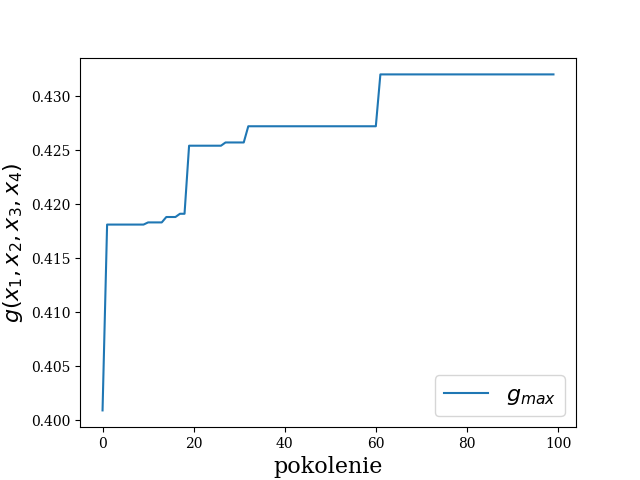
\includegraphics[width = 0.9\linewidth]{img/cnn_maxes_first}
	 \caption{Maksymalne wartości funkcji przystosowania w każdej iteracji dla sieci konwolucyjnych - podejście nr 1\\
              Źródło: praca własna}
	 \label{fig:cnn_maxes_first}
\end{figure}

\begin{figure}[h!tb]
	 \centering
	 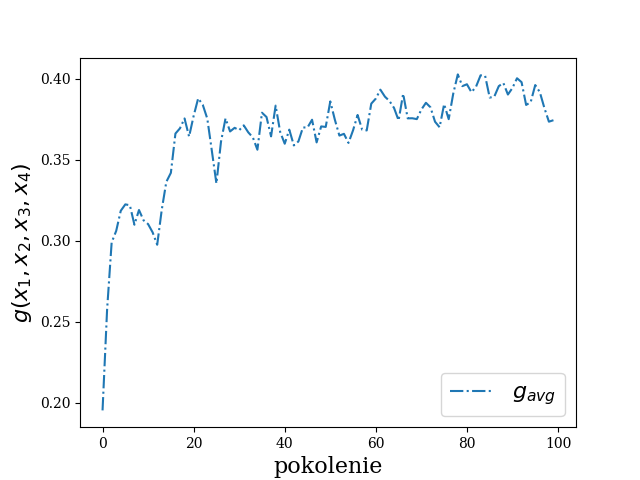
\includegraphics[width = 0.9\linewidth]{img/cnn_means_first}
	 \caption{Średnie wartości funkcji przystosowania w każdej iteracji dla sieci konwolucyjnych - podejście nr 1\\
              Źródło: praca własna}
	 \label{fig:cnn_means_first}
\end{figure}

Przeprowadzono dwa podejścia do tego eksperymentu, z powodu zaobserwowania niepokojących zjawisk w wynikach z podejścia pierwszego.
Na rys. \ref{fig:cnn_maxes_first} i rys. \ref{fig:cnn_means_first} obserwujemy wykresy odpowiednio najwyższych i średnich wartości funkcji przystosowania w populacji.

Badanie zostało przeprowadzone z ziarnem generatora 1337, jednak z przyczyn niezależnych algorytm przerywał działanie i był wzmnawiany odpowiednio w iteracjach 19, 27 i 54, zatem za każdym razem w tych momentach ziarno było ustawiane na 1337.

Przy pierwszym spojrzeniu nie widać nic niepokojącego.
Wykresy przedstawiają poprawne działanie algorytmu genetycznego.
Maksimum funkcji przysotoswania wg. algorytmu znajduje się w punkcie $\mathbf{x^*} = \begin{bmatrix}4 \\ 4 \\ 13 \\ 19\end{bmatrix}$ i zostało odnalezione w 62. iteracji.

Co widoczne będzie dopiero po porównaniu tych wykresów z wykresami na rys. \ref{fig:cnn_maxes} i rys. \ref{fig:cnn_means}, zarówno maksymalne jak i średnie wartości utrzymują się na niższym poziomie.
Jest tak ponieważ pojawiło się nadspodziewanie wiele wartości zbliżonych do 0.1, czego przyczyną może być jedno z następująych dwóch zjawisk:
\begin{enumerate}
  \item sieć ma bardzo złą strukturę (np. 1 filtr konwolucyjny przed warstwą agregującą)
  \item błędy w trakcie uczenia sieci przez węzeł obliczeniowy, które nie powodowały wyłączenia programu, jednak miały istotny wpływ na wynik
\end{enumerate}
Po bliższym przyjrzeniu się kilku przypadkom z danych znaleziono przykłady, w których sieć wygląda, jakby nie miała powodu by osiągać niskie wyniki, np. $\mathbf{x} = \begin{bmatrix}30 \\ 20 \\ 15 \\ 20\end{bmatrix}$, a  jej skutczność klasyfikacji była oceniana na poziomie 10\%.

Przyczyną okazało się złe skonfigurowanie węzłów obliczneniowych.
Wówczas korzystano z węzłów obliczeniowych opartych na obrazie \textit{Data Science Virtual Machine for Linux}.
Obraz ten został wybrany ze względu na preinstalowane biblioteki \textit{Keras, TensorFlow i Numpy}.
Po bliższym przyjrzeniu się sytuacji i ponownym uruchomieniu konkretnego przykładu na maszynie wirtualnej \textit{Data Science Virtual Machine for Linux} ukazało się wiele ostrzeżeń, jak na rys. \ref{fig:warnings}.

\begin{figure}[h!tb]
	 \centering
	 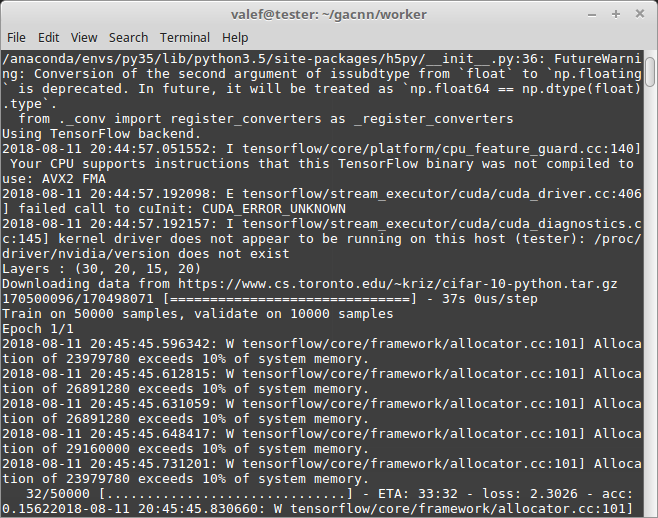
\includegraphics[width = 0.9\linewidth]{img/warnings}
	 \caption{Ostrzeżenia występujące w trakcie pracy węzła obliczeniowego  \\
              Źródło: praca własna}
	 \label{fig:warnings}
\end{figure}

Widać, że maszyna ma problem z alokacją odpowedniej ilości pamięci dla większych sieci, stąd niepoprawne wyniki na poziomie 10\% skuteczności klasyfikacji.
W trakcie pierwszego podejścia przyczynę problemu odnaleziono dopiero po wykonaniu powższych pomiarów.
To podejście okazało się być podejściem testowym i pomogło dopracować system w pełni, tak by działał poprawnie.
Łącznie uczenie wszystkich sieci trwało ok. 24 godzin na 20 węzłach.

Poniżej, na rys. \ref{fig:cnn_maxes} i rys. \ref{fig:cnn_means} przestawiono maksymalne i średnie wartości funkcji przystosowania dla kolejnych generacji w drugim podejściu do eksperymentu.
\begin{figure}[h!tb]
	 \centering
	 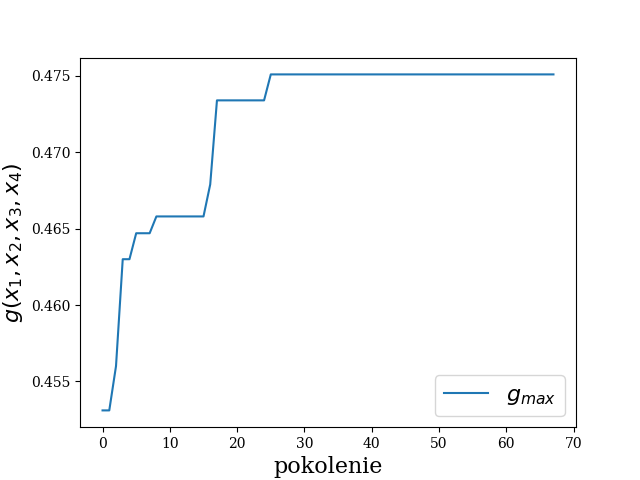
\includegraphics[width = 0.9\linewidth]{img/cnn_maxes}
	 \caption{Maksymalne wartości funkcji przystosowania w każdej iteracji dla sieci konwolucyjnych - podejście nr 2\\
              Źródło: praca własna}
	 \label{fig:cnn_maxes}
\end{figure}

\begin{figure}[h!tb]
	 \centering
	 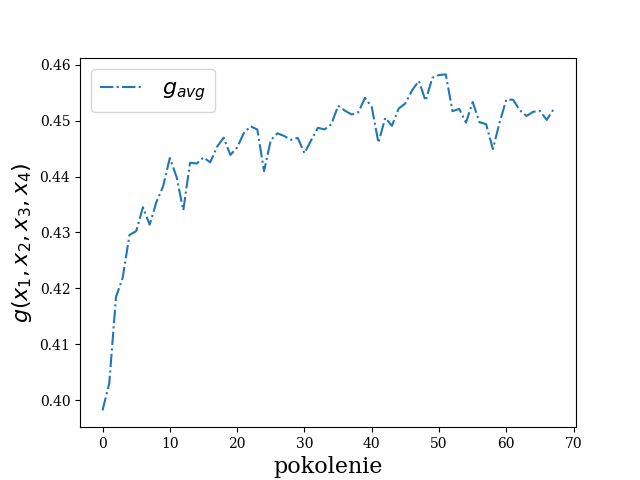
\includegraphics[width = 0.9\linewidth]{img/cnn_means}
	 \caption{Średnie wartości funkcji przystosowania w każdej iteracji dla sieci konwolucyjnych - podejście nr 2\\
              Źródło: praca własna}
	 \label{fig:cnn_means}
\end{figure}

Ponownie jak w teście Levego, wykresy maksymalnych i średnich wartości funkcji przystosowania osobników wyglądają jak typowy dla poprawnie zaimplementowanego algorytmu genetycznego.
Kryterium stopu które zadziałało tym razem to liczba iteracji bez poprawy - 50.
Znalezione przez algorytm rozwiązanie ma postać: $\mathbf{x^*} = \begin{bmatrix}12 \\ 21 \\ 23 \\ 31\end{bmatrix}$ i po jednej epoce uczenia osiąga skuteczność na poziomie 47.51\%.
Niestety, nie jesteśmy w stanie stwierdzić, czy jest to minimum globalne bez wykonywania kosztownego przeszukiwania metodą siłową.

Do drugiego podejścia wymieniono całą infrastukturę węzłów obliczeniowych, tj. zniszczono 20 maszyn wirtualnych opartych na obrazie \textit{Data Science Virtual Machine for Linux} i wymieniono je na obrazy \textit{Ubuntu Server 17.10}, jak opisano w \ref{sec:azure}.
Stwierdzono, że na żadnej z maszyn nie występują ostrzeżenia jak na rys. \ref{fig:warnings}.
Dodatkowo, w stosunku do poprzedniej próby wprowadzono modyfikacje w celu zaoszczędzenia czasu obliczniowego.
Od tego momentu opisany w \ref{sec:queue_system} rozpoczął wewnętrznie sprawdzać, czy powtarzają się osobniki do policzenia, aby nie liczyć ich kilka razy.

Dla drugiego uruchomienia przeprowadzono statystykę ile obliczeń zaoszczędzono.
Sumarycznie nauczono 3827 różnych sieci.
System zliczał liczbę duplikatów w każdej iteracji i przez całe swoje działanie zaoszczędził 501 obliczeń.
W stosunku do pełnej liczby 4328 wyznaczeń funkcji przystosowania uzyskaliśmy 10\% oszczędność czasu.
Dodatkowo, algorytm tym razem nie liczył pełnych 100 iteracji, tylko zakończył swoje działanie w iteracji nr 68 (przy braku poprawy o zadany próg od iteracji nr 18), co ostatecznie zaowocowało ok. 15 h pracy przy drugiej próbie.
Patrząc na wykres \ref{fig:cnn_maxes} widać, że poprawa wyniku pomiędzy 20 i 30 iteracją nie została uwzględniona jako poprawa, gdyż nie przekroczyła zadanego progu $\epsilon$.

\section{Porównanie wyników dla uczenia 1- i 10- epokowego}\label{sec:thesis_proof}
W tym przypadku również przeprowadzono eksperyment dla dwóch przypadków - z infrastukturą opartą na obrazach \textit{Data Science Virtual Machine for Linux} oraz na \textit{Ubuntu Server 17.10}.
Plan eksperymentu przedstawia się następująco:
\begin{enumerate}
  \item Z danych zebranych w badaniu \ref{sec:actual_experiment} wybierz najlepszego, średniego i najsłabszego osobnika w każdej iteracji
  \item Dokonaj uczenia owych osobników przez 10 epok
  \item Dla każdej trójki najlepszy-średni-najgorszy sprawdź, czy kolejność została zachowana
\end{enumerate}

Biorąc pod uwagę, że wszystkich możliwych ustawień trzech osobników jest $P_3 = 3! = 6$, jeżeli nie byłoby żadnego związku pomiędzy wynikiem uzyskanym po 1- a po 10- epokowym uczeniu, stosunek przypadków, w których kolejność została zachowana, do wszystkich przypadków powinien wynieść ok 16\%.

Dla przypadku, tj. węzły obliczeniowe utworzone na podstawie \textit{Data Science Virtual Machine for Linux} - jedynie w 3 przypadkach na 100 kolejność się zgadzała. Wynika to ze złego działania węzłów obliczeniowych - nie jesteśmy w stanie nic powiedzieć, ponieważ zbyt wiele wyników jest zniekształconych w wyniku braku pamięci.
Dla uczenia 10-epokowego jedynie 9 sieci na 156 uczonych uzyskało wynik powyżej 15\% - nie są to osiągi jakie powinna osiągać sieć po 10 epokach uczenia.

Dla przypadku drugiego, tj. infrastuktura oparta o \textit{Ubuntu Server 17.10}, czyli, jak stwierdzono w \ref{sec:actual_experiment} działającej metody obliczania wartości funkcji przystosowania, liczba iteracji dla których kolejność została zachowana wyniosła 40 na 68, co stanowi około 59\%.
Wynik ten jest dużo wyższy niż losowe ustalanie kolejności (poziom 16\%).
Pozwala to wysnuć wniosek, że istnieje pewien związek pomiędzy osiągami sieci po 1-epoce uczenia a ostatecznymi osiągami (tutaj rozumianymi jako 10-epokowe uczenie), gdyż szansa, że trzy sieci zachowają swoją kolejność pod względem jakości klasyfikacji wynosi niemalże 60 \%.
Co więcej, dla prostszego testu, to jest bez uwzględnienia środkowego środkowego osobnika, uszeregowanie zgadzało się w 100 \% przypadków, tj. najlepsza sieć była najlepsza zarówno po 10 jak i 1 epoce uczenia, a najgorsza pozostwała najgorszą.

Tutaj również, jak w \ref{sec:actual_experiment} dokonano ulepszenia pomiędzy uruchomieniami algorytmu.
W celu lepszej wizualizacji zachowania sieci w trakcie uczenia, zapisywano historię uczenia, tj. wartości funkcji przystosowania i funkcji kosztu w każdej epoce uczenia uzyskane na zbiorze uczącym oraz uzyskane na zbiorze testowym.
Dzięki temu ulepszeniu można zobaczyć przebieg uczenia dowolnej sieci z arbitralnie wybranej iteracji algorytmu.

\section{Porównanie przebiegu uczenia sieci w pierwszej i ostatniej iteracji algorytmu genetycznego}
Celem tego badania jest sprawdzenie jak zmienia się dynamika uczenia sieci w zależności od jej struktury uzyskanej w wyniku działania algorytmu genetycznego.
Aby zobrazować różnice pomiędzy owymi sieciami zestawiono ze sobą przebiegi uczenia:
\begin{enumerate}
  \item Najlepszej, środkowej i najgorszej sieci z populacji inicjalnej (rys. \ref{fig:iter_learn_first})
  \item J.w. sieci z populacji końcowej (rys. \ref{fig:iter_learn_last})
  \item Najlepszej sieci z pierwszej i ostatniej iteracji algorytmu genetycznego (rys. \ref{fig:iter_learn_best})
\end{enumerate}
Co zaobserwowano:
\begin{itemize}
  \item Wszystkie krzywe uczenia ewolują w ten sam sposób - z każdą epoką uczenia coraz lepiej klasyfikują obrazy
  \item Porównując rys. \ref{fig:iter_learn_first} i rys. \ref{fig:iter_learn_last} widzimy, że w obydwu przypadkach najlepsza i średnia sieć znajdują się blisko siebie, a najgorsza znajduje się stosunkowo daleko pod nimi.
  \item Na rys. \ref{fig:iter_learn_last} widzimy sytuację, w której w dalszych fazach uczenia sieć średnia wyprzedza początkowo najlepszą.
  Zgodnie z \ref{sec:thesis_proof}, do takich sytuacji dochodzi w 40\% iteracji algorytmu.
  Należy przy tym zauważyć, że przecinają się linia średnia z najlepszą, a linia najgorsza pozostaje w bezpiecznej odległości przez kolejne epoki.
  Nasuwa się przy tym wniosek, że im większa początkowa (po jednej epoce) różnica w jakości klasyfikacji obrazów przez sieć, tym większe prawdopodobieństwo, że po pełnym uczeniu relacja pomiędzy jakościami sieci się nie zmieni.
  \item Porównując rys. \ref{fig:iter_learn_first} z rys. \ref{fig:iter_learn_last} lub patrząc na przebiegi na rys. \ref{fig:iter_learn_best} widzimy, że działanie algorytmu genetycznego podnosi pułap, na którym znajdują się krzywe uczenia.
  Wartości zarówno w 1. jak i 10. epoce znajdują się wyżej w iteracji ostatniej niż pierwszej.

\end{itemize}

\begin{figure}[h!tb]
	 \centering
	 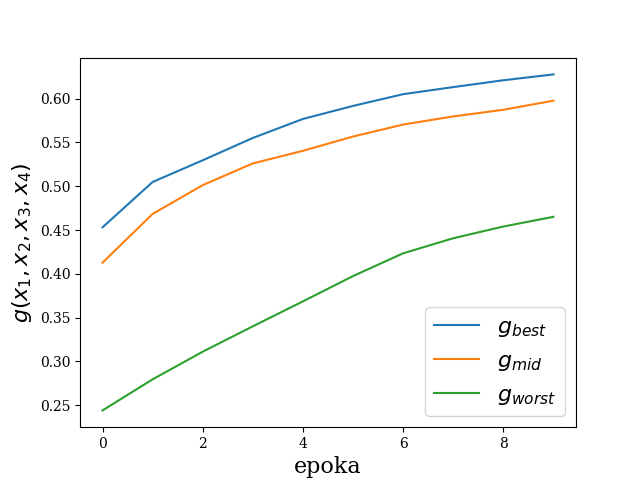
\includegraphics[width = 0.85\linewidth]{img/iter_learn_first}
	 \caption{Przebieg uczenia najlepszej, średniej i najgorszej sieci w pierwszej iteracji algorytmu genetycznego\\
              Źródło: praca własna}
	 \label{fig:iter_learn_first}
\end{figure}

\begin{figure}[h!tb]
	 \centering
	 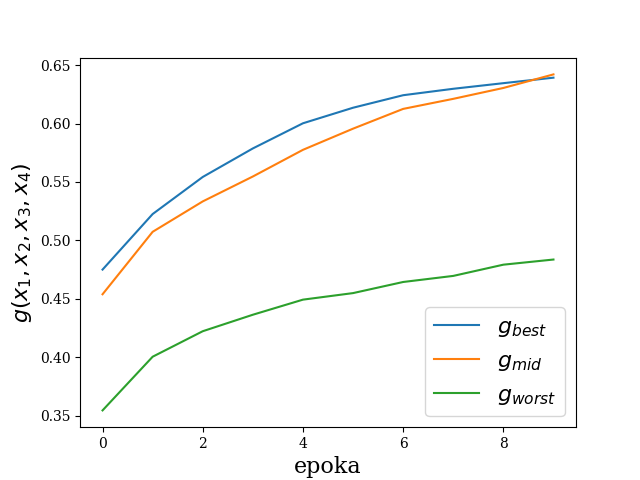
\includegraphics[width = 0.85\linewidth]{img/iter_learn_last}
	 \caption{Przebieg uczenia najlepszej, średniej i najgorszej sieci w ostatniej iteracji algorytmu genetycznego\\
              Źródło: praca własna}
	 \label{fig:iter_learn_last}
\end{figure}

\begin{figure}[h!tb]
	 \centering
	 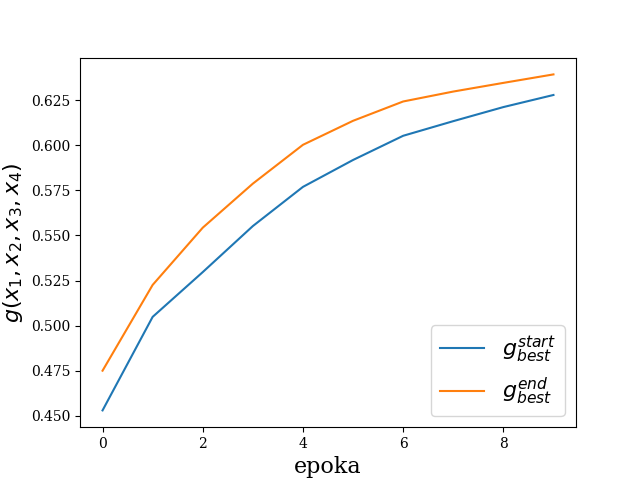
\includegraphics[width = 0.85\linewidth]{img/iter_learn_best}
	 \caption{Przebieg uczenia najlepszej sieci w pierwszej i ostatniej iteracji algorytmu genetycznego\\
              Źródło: praca własna}
	 \label{fig:iter_learn_best}
\end{figure}

Ostatecznie widoczne jest polepszenie procesu uczenia sieci przez algorytm genetyczny.
Nie jest to polepszenie w sensie dynamicznym, gdyż kształt funkcji uczenia prawie się nie zmienia, jednakże w sensie statycznym, czyli wartości na początku i na końcu, widać poprawę.

\section{Osiągi najlepszej według algorytmu sieci po 25 epokach uczenia}\label{sec:25_epoch_training}
\begin{figure}[h!tb]
	 \centering
	 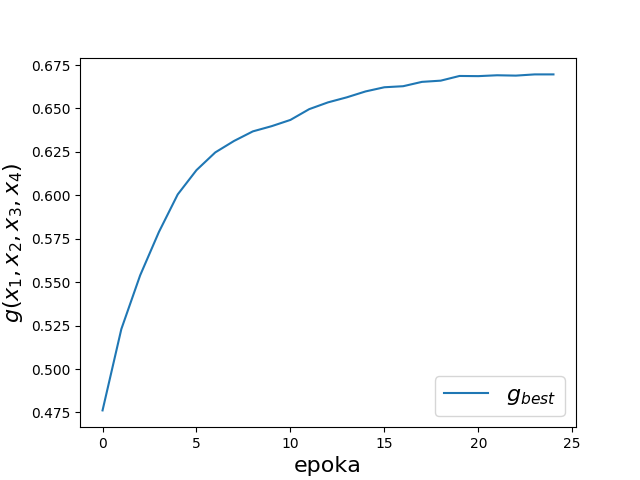
\includegraphics[width = 0.85\linewidth]{img/25epoch}
	 \caption{Przebieg uczenia najlepszego osobnika z \ref{sec:actual_experiment} dla 25 epok\\
              Źródło: praca własna}
	 \label{fig:25epoch}
\end{figure}


Dla rozwiązania $\mathbf{x^*} = \begin{bmatrix}12 \\ 21 \\ 23 \\ 31\end{bmatrix}$ przeprowadzone zostanło uczenie 25-epokowe.
Na rys. \ref{fig:25epoch} przedstawiono krzywą uczenia dla tego przypadku:

Ostateczny wynik uzyskany przez sieć to 67\%.
Jest to gorszy wynik, niż w przykładzie, na którym oparto budowanie modeli sieci i uczenie ich (dostępny pod adresem \url{https://github.com/keras-team/keras/blob/master/examples/cifar10_cnn.py})
Powodem tego może być brak zastosowania warstw \textit{dropout} w sieci modyfikowanej przez algorytm genetyczny, co prowadzi do nadmiernego dopasowania.
Dalsza opytmalizacja powyżej uzyskanych 67\% wymagałaby modyfikacji elementów przyjętych jako stałe w strukturze sieci.
Wynik ten jest jednak optymalny przy tak narzuconej strukturze.

\chapter{Podsumowanie}\label{chap:summary}

Badanie zależności pomiędzy początkową wydajnością uczonych sieci a ich wynikami po pełnym uczeniu okazało się kosztowne i czasochłonne.

Na samym początku wymagało pogłębienia wiedzy o:

\begin{itemize}
  \item uczeniu maszynowym,
  \item meta uczeniu,
  \item uczeniu z nadzorem,
  \item klasyfikacji obrazków,
  \item zbiorze CIFAR-10,
  \item metodzie k-najbliższych sąsiadów,
  \item klasyfikatorach liniowych,
  \item sieciach neuronowych - ogólnie,
  \item konwolucyjnych sieciach neuronowych,
  \item algorytmie genetycznym.
\end{itemize}

Z takim przygotowaniem teoretycznym można było podejść do zaprojektowania systemu do przeprowadzenia badań.
To z kolei wiązało się z kolejnymi krokami:

\begin{enumerate}
  \item redukcji problemu, to jest dokładniejszego zdefiniowania problemu z uwzględnieniem ograniczonego czasu i budżetu na obliczenia,
  \item zdefiniowania osobnika dla algorytmu genetycznego jako sieci neuronowej o określonej strukturze z pewnymi zmiennymi parametrami,
  \item zdefiniowaniu konkretnych operacji genetycznych jakie przeprowadzane będą w tej konkretnej implementacji algorytmu genetycznego, a konkretniej zdefiniowanie:
  \begin{itemize}
    \item krzyżowania,
    \item mutacji,
    \item upewnienia się, że osobniki znajdują się wewnątrz zdefiniowanej przestrzeni poszukiwań,
    \item substytucji między pokoleniami.
  \end{itemize}
  \item zaprojektowaniu ogólnej architektury oprogramowania do przeprowadzenia eksperymentu,
  \item zdefiniowaniu sposobu pracy węzła zarządzającego przeprowadzaniem eksperymentu,
  \item zaprojektowaniu systemu kolejkowania zadań w celu przyspieszenia obliczeń,
  \item stworzeniu protokołu do komunikacji z węzłami zdalnymi,
  \item implementacji węzła obliczeniowego wykonującego zlecone mu zadania i zwracającego wyniki,
  \item automatyzacji tworzenia nowych węzłów obliczeniowych,
  \item analizie możliwości replikacji wyników badań ze względu na korzystanie z generatora liczb pseudolosowych.
\end{enumerate}

Powstawanie owego systemu wymagało czasu, dogłębnego przemyślenia oraz pochłonęło zasoby na zarówno udane jak i nieudane próby przeprowadzenia eksperymentu.
Ostatecznie testy i wyniki, które zostały przeprowadzone można podsumować następująco:

\begin{itemize}
  \item przeprowadzono badanie wariancji wyników dla sieci o jednej strukturze przy rożnych wartościach ziarna generatora losowego w celu wyznaczenia progu poprawy pomiędzy iteracjami,
  \item przeprowadzono test działania algorytmu genetycznego dla testowej funkcji Levy'ego, na podstawie którego wyciągnięto wniosek, że algorytm genetycznie działa poprawnie i można go zastosować do właściwego zadania zmieniając wyznaczaną funkcję celu,
  \item przeprowadzono test działania systemu kolejkowego dla jednej maszyny lokalnej, z którego wynikła konieczność zmiany długości bufora dla przesyłu danych pomiędzy węzłami
  \item przeprowadzono poszukiwanie optymalnej struktury sieci neuronowej za pomocą algorytmu genetycznego w dwóch próbach, gdzie na podstawie pierwszej naprawiono błędy w systemie, a obserwując wykresy wyciągnięto wniosek, że uzyskiwana jakość sieci polepsza się (dowód tezy głównej)
  \item porównano wyniki dla uczenia 1- i 10- epokowego i na tej podstawie stwierdzono, że istnieje pomiędzy nimi związek (dowód tezy pomocniczej)
  \item zaobserwowano proces uczenia dla wybranych z pierwszej i ostatniej iteracji algorytmu genetycznego i porównano je, po raz kolejny obserwując polepszenie jakości sieci, a zatem optymalizację struktury (dowód tezy głównej)
  \item uzyskaną w wyniku działania algorytmu genetycznego sieć uczono przez 25 epok jako pełne uczenie i wyciągnięto wniosek, że proponowane stałe elementy struktury sieci mogłyby być lepiej dobrane
\end{itemize}

W toku przeprowadzonych badań udało się potwierdzić obydwie stawiane we wstępie tezy, tj.

\begin{enumerate}
  \item możliwa jest optymalizacja struktury konwolucyjnych sieci neuronowych za pomocą algorytmu genetycznego (teza główna),
  \item istnieje związek pomiędzy skutecznością sieci po krótkim i długim uczeniu (teza pomocnicza).
\end{enumerate}

Tym samym cel pracy został zrealizowany.

System można w dalszym ciągu dopracować.
Poniżej przedstawiono kilka propozycji ulepszeń:

\begin{itemize}
  \item aby zapewnić możliwość replikacji badań zrezygnowano z równoległych obliczeń na GPU i system dostosowany został do obliczeń na CPU, można by jednak uwzględnić taką możliwość w kolejnych generacjach systemu,
  \item system kolejkowy można by dodatkowo usprawnić implementując algorytm rozdzielania zadań dla równoległych maszyn, np. implementując algorytm CDS (Campbella, Dudeka i Smitha),
  \item można w dalszym ciągu ulepszyć czytelność kodu przepisując odpowiednie fragmenty,
  \item algorytmy parametry genetycznego dobrane zostały metodą prób i błędów - można by wejść na kolejny poziom meta uczenia również dobierając jego parametry za pomocą innego algorytmu uczenia maszynowego,
  \item ustalone elementy sieci neuronowej (stałą część jej struktury) można by ulepszyć tak, by ostateczna wynikowa sieć miała lepsze wyniki klasyfikacji,
  \item węzły zdalne w żaden sposób nie sprawdzają, kto wysyła im zadania.
  Może to doprowadzić do sytuacji gdzie uruchomienie jednocześnie kilku systemów kolejkowych zlecających zadanie uniemożliwia poprawne działanie systemu.
  Należałoby to poprawić w przypadku korzystania z systemu przez więcej niż jedną osobę.
\end{itemize}

Dodatkowo pojawiło się nowe pytanie: jaki wpływ ma początkowa różnica w skuteczności klasyfikacji przez sieć jednoepokową na tę samą różnicę dla 10-epok?
Widać zatem, że można dalej prowadzić badania w tym kierunku i pozostało wiele pola do badań w dziedzinie dobierania optymalnej struktury konwolucyjnuych sieci neuronowych.

\input{Chapter6}
% .

\clearpage

\bibliography{bibl}{}
\bibliographystyle{plain}

%spis rysunków
\clearpage
\listoffigures

%spis tablic
\clearpage
\listoftables

\end{document}